\chapter{LTL Bitmap}

\section{Introduction}\label{sec:intro} %% {{{

\emph{Temporal logic} \cite{huth2004} is a logistic system which uses rules and symbols to describe and reason about the change of a system's state in terms of time. It is based on the idea that one state may not be constantly true or false as time goes. \emph{Linear Temporal Logic (LTL)} \cite{pnueli97} is a temporal logic, and as its name entails, \emph{LTL} can denote only one sequence of states and for each state there is only one future state.

\emph{Bitmap}, also known as \emph{bit array} or \emph{bitset}, is a compact data structure storing 0 or 1 bits. It can be used to express a set of numbers, or an array where each bit represents a 2-values option. In this paper, we explore the idea of integrating the bitmap manipulations with the calculation of LTL formulas. For this purpose, in Section \ref{sec:ltlbitmap}, we introduce a solution to map LTL's atomic propositions into bits, and then design the algorithms to implement the LTL operators with the bitmap operations.

A bitmap having consecutive 0s or 1s can be compressed. Bitmap compression is able to reduce the space cost and speed up the operation \cite{lemire2014}. Section \ref{sec:compression} shows several bitmap compression algorithms and discusses the impact of compressed bitmap on the performance of our solution. 

%% }}} --- Section

\section{Bitmap compression}\label{sec:compression} %% {{{

For the bitmap mapping from the states, the result bitmap of certain operators tend to have longer runs of consecutive 0s or 1s than the input ones. The operators \textbf{F} and \textbf{G} output the bitmap which has at most two sequences of consecutive 0s or 1s. The operators \textbf{U}, \textbf{W} and \textbf{R} are able to combine the continuous 1s from the two input bitmaps to get a longer sequence of 1s and also to filter out the discontinuous 1s to get a longer sequence of 0s. Thus we introduced bitmap compression in our solution to see if it can improve the performance of our solution.

There are many popular compression algorithms are based on the Running Length Encoding (RLE) model derived from BBC\cite{antoshenkov1995byte}. We choose WAH\cite{wu2006optimizing}, Concise\cite{colantonio2010} and EWAH\cite{lemire2010} because they have well-implemented Open Source libraries in Java. These algorithms share some common features and also have their own characters:
\begin{itemize}
\item All of them have two different kinds of words, one of which is to store the raw uncompressed word (literal word) and the other is compressed word (sequence word) having a bit and a number. The number represents the number of consecutive words which are full of 0s or 1s determined by the bit.
\item \emph{WAH} and \emph{Concise} use the most significant bit to mark if the current word is compressed or uncompressed.
\item \emph{EWAH} does not have this kind of bit, so it has to save the number of following uncompressed words, which causes that it is impossible to reversely enumerate the bits from back to front, because the type of each word cannot be detected directly. However, it can use all bits of a literal word to store data.
\item \emph{Concise} consumes 5 bits in every compressed word to store the position of a "flipped" bit which flips the corresponding bit of the first full word. As \cite{colantonio2010} says, this feature can improve the compression ratio in the worst case.
\item Table \ref{tbl:bmparms} lists the parameters of the RLE-model algorithms:
\begin{itemize}
  \item The number of a word ($wlen$);
  \item The number of available bits in a literal word ($ulen$);
  \item The max number of bits stored in a sequence word ($wcap$);
\end{itemize}
\end{itemize}

\begin{table}[h]
\centering
\begin{tabular}{|c|c|c|c|}
\hline
& ulen & wlen & wcap \\
\hline
WAH & 31 bits & 32 bits & $2^{30} - 1$ \\
\hline
Concise & 31 bits & 32 bits & $2^{25} - 1$ \\
\hline
EWAH & 32 or 64 bits & 32 or 64 bits & $2^{16} - 1 \text{ or } 2^{32} - 1$ \\
\hline
\end{tabular}
\caption{Parameters of RLE-model algorithms}
\label{tbl:bmparms}
\end{table}

Considering that a $n$-bits bitmap has $m$ sequences of consecutive (0...1...) bits:
\begin{align*}
& c^1_0c^0_1c^1_1c^0_1c^1_2c^0_2...c^1_{m - 1}c^0_{m - 1}, c^i_j \text{ is the number of } \\
& \text{consecutive } i \text{ bits and } i \in (0, 1),\, 0 \leq j \leq m.  
\end{align*}

Then the number of total bits, i.e. the size of the uncompressed bitmap is:
\begin{align*}
& total\_bits = \sum_{j = 0}^{m - 1} \sum_{i = 0}^1 c^i_j = \sum_{j = 0}^{m - 1} \sum_{i = 0}^1 l^i_j + s^i_j, \\
& l^i_j = c^i_j \text{ mod } ulen, s^i_j = c^i_j - l^i_j
\end{align*}

If exists a positive integer $slen$, $\forall c^i_j = slen$, then
\begin{align}
m = n \div (2 \times slen) \label{eq:seqnum}
\end{align}

When $1 \leq slen < wlen$, then $\forall l^i_j > 0, \forall s^i_j = 0$, which is considered the worst case, the size of the compressed bitmap is:
\begin{align*}
compressed\_bits = \lceil \frac{total\_bits}{ulen} \rceil \times wlen 
\end{align*}

None of the three RLE-model algorithms can well compress this kind of bitmap. Both \emph{WAH} and \emph{Concise} waste one bit for the type identification and \emph{EWAH} seems to cost the least for its $ulen = wlen$ but its actual size should be a little more because some empty sequence word is needed to store the number of the literal words.

Furthermore, when $wlen \leq slen$, then $\forall s^i_j > 0$, the sequence can be compressed with any RLE-model algorithm. Suppose $\forall l^i_j > 0$, the size of the compressed bitmap is:
\begin{align*}
compressed\_bits = &\sum_{j = 0}^{m - 1} \sum_{i = 0}^1 \lceil \frac{slen}{wcap} \rceil \times wlen + wlen \\
= & 2 \times m \times wlen \times (1 + \lceil \frac{slen}{wcap} \rceil)
\end{align*}

Section \ref{sec:ltlbitmap} mentions that the time and space complexities of all LTL operators are $O(n)$ where $n$ is the size of the input uncompressed bitmap. After applying RLE-model bitmap compression algorithms to our solution, the space complexities become $O(m)$ as is discussed above, and we managed to make the time complexities also become $O(m)$ by implementing the bitmap manipulation functions listed in Table \ref{tbl:bmhelpers} for every  bitmap compression algorithms.

Because of lack of the support of random access, we cannot enumerate the bits in the same way as uncompressed bitmap. Therefore we design an \emph{iterator} data structure to store not only the absolute index of current bit in the uncompressed bitmap but also the relative index in the compressed bitmap.

Taking the function \textbf{next1()} as an example, if the current relative index is in a sequence word of 0, the search in this word is unnecessary, and we just jump to the next word; if the index is in a sequence word of 1, we return the current index; however, if the index is in a literal word, we have to look for the bit 1 in the $ulen$-bits word.

Besides the RLE-model algorithms, there are other bitmap compression model which supports fast random access like the uncompressed bitmap does. One of them is Roaring bitmap\cite{lemire2015}.

Roaring bitmap splits 32-bit indexes into chunks, each of which stores the 16 most significant bits of a 32-bit integer and points to a specialized container storing the 16 least significant bits. There are two types of containers: a sorted 16-bit integer array for \emph{sparse} chunks which store at maximum 4096 integers, and a bitmap for \emph{dense} chunks which store $(4096, 2^{16})$ integers. The time complexities of the LTL operators with \emph{Roaring bitmap} are $O(n)$ because we cannot skip certain bits when enumerating the bitmap.

%% }}} --- Section

\section{Calculate LTL formulas with Bitmap}\label{sec:ltlbitmap} %% {{{

In this section we introduce our solution of mapping LTL states to bitmaps and calculating the formulas with the mapped bitmaps.

\subsection{Background and related works} %% {{{

A well-formed \emph{LTL} formula consists of a finite set of atomic propositions $Props$, propositional logic operators $\neg, \wedge, \vee, \rightarrow$ and temporal logic operators \textbf{F}(future), \textbf{G}(global), \textbf{X}(next), \textbf{U}(until), \textbf{W}(weak-until) and \textbf{R}(release). It can be defined as follows:
\begin{enumerate}
  \item Every atomic proposition $p$ of the finite set is a formula;
  \item If $\psi$ is a formula, then so are $\neg\psi$, $\mathop{F}\psi$, $\mathop{G}\psi$, $\mathop{X}\psi$;
  \item If $\psi$ and $\varphi$ are formulas, then so are $\psi\wedge\varphi$, $\psi\vee\varphi$, $\psi\mathrel{U}\varphi$, $\psi\mathrel{W}\varphi$, $\psi\mathrel{R}\varphi$.
\end{enumerate}

For a sequence of states $s_0, s_1, s_2, ..., s_i, s_{i + 1}, ...$ where $s_{i + 1}$ is a future state of $s_i$, we define a path with $\pi^i = s_i \rightarrow s_{i + 1} \rightarrow ...$ where $i$ is the first state in this path. Given that $\pi(i)$ is the set of atomic propositions which are true at the $i$th state, whether a path $\pi^i$ satisfies an \emph{LTL} formula is defined as follows:
\begin{itemize}
  \item \listequation{\pi^i \vDash p \iff p \in \pi(i)} \label{eq:ap}
  \item \listequation{\pi^i \vDash \neg\psi \iff \pi^i \nvDash \psi} \label{eq:not}
  \item \listequation{\pi^i \vDash \psi \wedge \varphi \iff \pi^i \vDash \psi$ and $\pi^i \vDash \varphi} \label{eq:and}
  \item \listequation{\pi^i \vDash \psi \vee \varphi \iff \pi^i \vDash \psi$ or $\pi^i \vDash \varphi} \label{eq:or}
  \item \listequation{\pi^i \vDash \psi \rightarrow \varphi \iff \pi^i \vDash \varphi$ whenever $\pi^i \vDash \psi} \label{eq:then}
  \item \listequation{\pi^i \vDash \mathop{X}\psi \iff \pi^{i + 1} \vDash \psi} \label{eq:next}
  \item \listequation{\pi^i \vDash \mathop{G}\psi \iff \forall j \geq i, \pi^j \vDash \psi} \label{eq:global}
  \item \listequation{\pi^i \vDash \mathop{F}\psi \iff \exists j \geq i, \pi^j \vDash \psi} \label{eq:future}
  \item \listequation{\pi^i \vDash \psi \mathrel{ U } \varphi \iff \exists j \geq i, \pi^j \vDash \varphi$ and $\forall k, i \leq k < j, \pi^k \vDash \psi} \label{eq:until}
  \item \listequation{\pi^i \vDash \psi \mathrel{ W } \varphi \iff$ either $\exists j \geq i, \pi^j \vDash \varphi$ and $\forall k, i \leq k < j, \pi^k \vDash \psi$, or $\forall k \geq i, \pi^k \vDash \psi} \label{eq:wuntil}
  \item \listequation{\pi^i \vDash \psi \mathrel{ R } \varphi \iff$ either $\exists j \geq i, \pi^j \vDash \psi$ and $\forall k, i \leq k \leq j, \pi^k \vDash \varphi$, or $\forall k \geq i, \pi^k \vDash \varphi} \label{eq:release}
\end{itemize}

\todokun{On va raccourcir cette section. LTL est bien connu des gens de la conférence.}

%% }}} --- Subsection

\subsection{Manipulate bitmaps to implement LTL operators} %% {{{

Given a finite $n$-states sequence of states $(s_0, s_1, ..., s_{n - 1})$ and an LTL formula $L$, a $n$-bits bitmap defined as Definition \eqref{eq:map} is dedicated to store the bits which indicate whether the corresponding paths satisfy the formula. The bitmap mapping from the formula $L$ is called $B_l$.

\begin{equation}\label{eq:map}
(b_0b_1...b_ib_{i + 1}...b_{n - 1})_n, b_i = \begin{cases}
1, & \text{if $\pi^i \vDash L$} \\
0, & \text{otherwise}
\end{cases}
\end{equation}

We suppose that a well-designed data structure of bitmap has certain functions as are described in Table \ref{tbl:bmfuncs}.
\begin{table}[h]
\centering
\begin{tabular}{|l|l|}
\hline
Function & Description \\
\hline
size(bitmap) & gets the size of the bitmap. \\
\hline
get(bitmap, index) & gets the true/false value from the specific index in the bitmap. \\
\hline
set(bitmap, index, val) & sets the true/false value to the specific index in the bitmap. \\
\hline
and(bitmap1, bitmap2) & performs a logic $\mathit{AND}(\wedge)$ operation of the two input bitmaps. \\
\hline
or(bitmap1, bitmap2) & performs a logic $\mathit{OR}(\vee)$ operation of the two input bitmaps. \\
\hline
not(bitmap) & performs a logic $\mathit{NOT}(\neg)$ operation of the input bitmap. \\
\hline
\end{tabular}
\caption{Basic bitmap functions}
\label{tbl:bmfuncs}
\end{table}

These bitmap functions are enough to implement the LTL operators, but in order to optimize our solution and integrate with bitmap compression algorithms shown in Section \ref{sec:compression}, we need to manipulate the internal data structure of the bitmap and thus introduce 7 derivative bitmap functions (See Table \ref{tbl:bmhelpers}).
\begin{table}[h]
\centering
\begin{tabular}{|l|p{8cm}|}
\hline
Function & Description \\
\hline
addMany(bitmap, val, len) & adds a $len$-bits sequence of the same value to the end of the bitmap whose size then increases by $len$. \\
\hline
copyTo(bitmapDest, bitmapSrc, start, len) & copies the $len$-bits sequence from the index $start$ in bitmap $bitmapSrc$ to the end of another bitmap $bitmapDest$ whose size then increases by $len$. \\
\hline
removeFirstBit(bitmap) & removes the first bit of the bitmap, and the size of the bitmap decreases by 1. \\
\hline
next0(bitmap, start) & gets the position of the next occurrence of the bit "0" from the inclusive position $start$ of the bitmap, or -1 if there is no more "0". \\
\hline
next1(bitmap, start) & gets the position of the next occurrence of the bit "1" from the inclusive position $start$ of the bitmap, or -1 if there is no more "1". \\
\hline
last0(bitmap) & gets the position of last occurrence of the bit "0" in the bitmap, or -1 if the bitmap does not have a bit "0". \\
\hline
last1(bitmap) & gets the position of last occurrence of the bit "1" in the bitmap, or -1 if the bitmap does not have a bit "1". \\
\hline
\end{tabular}
\caption{Derivative bitmap functions}
\label{tbl:bmhelpers}
\end{table}

The finite set of atomic propositions constitute the initial bitmaps. Consider a $n$-states sequence, according to Definition \eqref{eq:ap}, the bit $b_i$ of $B_p$ is set to $1$ if the atomic proposition is true at the corresponding state $s_i$, otherwise 0.

Propositional logic operators are translated to bitwise operators. The functions $\mathop{not}(), \mathop{and}(), \mathop{or}()$ from the bitmap are enough to the calculation of the formulas $\neg\psi$\eqref{eq:not}, $\psi \wedge \varphi$\eqref{eq:and}, $\psi \vee \varphi$\eqref{eq:or}. And the formula $\psi \rightarrow \varphi$ can be expanded to $\neg \psi \vee \varphi$ \cite{huth2004}.

\begin{align*}
\neg \psi &\mapsto \mathop{not}(B_\psi) \\
\psi \wedge \varphi &\mapsto \mathop{and}(B_\psi, B_\varphi) \\
\psi \vee \varphi &\mapsto \mathop{or}(B_\psi, B_\varphi) \\
\psi \rightarrow \varphi &\mapsto \mathop{or}(\mathop{not}(B_\psi), B_\varphi) \\
\end{align*}

Temporal logic operators are a little more complicated because they concern the change of the states in terms of time, therefore we have to enumerate the actual states and the bits in the bitmaps.

Definition \eqref{eq:next} states that the operator $\mathop{X}$ aims to check if the next state of a state is fine, so for a sequence of states, we just need to remove the first state and the rest states immediately become the "next" states. For the corresponding bitmap, we remove its first bit (see Algorithm \ref{alg:next}).

\begin{figure}
\centering
\subfloat[$\mbox{\bf X}\,\varphi$]{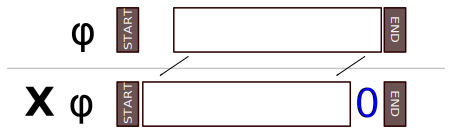
\includegraphics[scale=0.3]{Pattern-X}}~~~
\subfloat[$\mbox{\bf G}\,\varphi$]{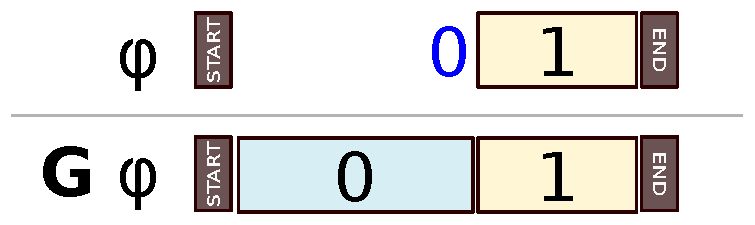
\includegraphics[scale=0.3]{Pattern-G}}~~~
\subfloat[$\varphi\,\mbox{\bf U}\,\psi$]{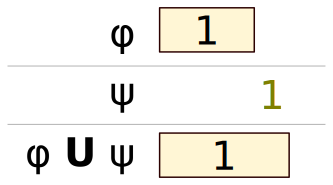
\includegraphics[scale=0.3]{Pattern-U}}
\caption{A graphical representation of the computation of three temporal operators on bitmaps}
\label{fig:patterns}
\end{figure}

\todokun{1. Il y a un problème avec l'algo suivant. Chaque opérateur doit retourner un vecteur de même longueur que l'entrée. Ici, X(10101) = (01010). On fait un left shift et on ajoute un zéro à la fin.

2. La mise en page des algorithmes n'est pas très belle. Utilise plutôt les packages algorithm et algpseudocode.

3. Tu peux supprimer Input, Output et le Begin/End principal de chaque algo.}

\begin{algo}[caption=ne\textbf{\textbf{X}}t, label={alg:next}]
Input: Bitmap $a$
Output: Bitmap
Begin
  if size($a) \leq 1$
    return empty Bitmap
  else
    // X(10101) $\Rightarrow$ (0101)
    $answer \gets$ removeFirstBit($a$)
    return $answer$
  endif
End
\end{algo}

The dual formulas $\mathop{G}\psi$ and $\mathop{F}\psi$ demand to find the $i$-th path $\pi^i$ from which on all the following paths $\pi^{i + 1}, \pi^{i + 2}, ... \pi^n$ relatively satisfy or do not satisfy the formula $\psi$, according to Definition \eqref{eq:global} and \eqref{eq:future}. Thus to implement these two formulas with bitmap, we need to do a search in the bitmap $B_{\psi}$ from back to front to find the last occurrence of the bit "0" or "1", as can be seen from Algorithm \ref{alg:global} and \ref{alg:future}.

\begin{algo}[caption=\textbf{G}lobal, label={alg:global}]
Input: Bitmap $a$
Output: Bitmap
Begin
  // G(101011) $\Rightarrow$ (000011)
  $pos \gets$ last0($a$)
  if $pos = -1$ then
    return $a$
  else
    $answer \gets$ empty Bitmap
    $s \gets$ size($a$)
    addMany($answer$, 0, $pos + 1$)
    addMany($answer$, 1, $s - pos - 1$)
    
    return $answer$
  endif
End
\end{algo}

\begin{algo}[caption=\textbf{F}uture, label={alg:future}]
Input: Bitmap $a$
Output: Bitmap
Begin
  // F(010100) $\Rightarrow$ (111100)
  $pos \gets$ last1($a$)
  if $pos = -1$ then
    return $a$
  else
    $answer \gets$ empty Bitmap
    $s \gets$ size($a$)
    addMany($answer$, 1, $pos + 1$)
    addMany($answer$, 0, $s - pos - 1$)
    
    return $answer$
  endif
End
\end{algo}

According to Definition \eqref{eq:until}, if there is a $\pi^j$ which satisfies $\varphi$ and the paths $\pi^i, \pi^{i + 1}, ... \pi^{j - 1}$ all satisfy $\psi$, the path $\pi^i$ must satisfy the formula $\psi \mathrel{U} \varphi$. With respect to the operation of bitmaps, we need to keep checking if there is any bit set as 1 in $B_{\psi}$ before the every occurrence of bit 1 in $B_{\varphi}$ (see Algorithm \ref{alg:until}).

\todokun{Algo ci-dessous: comme les entrées et les sorties sont toujours de même taille, le premier if n'est pas nécssaire.}

\begin{algo}[caption=\textbf{U}ntil, label={alg:until}]
Input: Bitmap $a$ and $b$
Output: Bitmap
Begin
  if size($a$) $\neq$ size($b$) then
    $dif\hspace{-0.1em}f \gets$ size($a$) $-$ size($b$)
    if $dif\hspace{-0.1em}f < 0$ then
      addMany($a$, 0, $-dif\hspace{-0.1em}f$)
    else
      addMany($b$, 0, $dif\hspace{-0.1em}f$)
    endif
  endif

  $answer \gets$ empty Bitmap
  $pos \gets 0$
  $size \gets$ size($a$)

  $a_1 \gets 0$
  $a_0 \gets 0$
  $b_1 \gets 0$
  $b_0 \gets 0$
  while $pos < size$ do
  begin
    if $a_1 \leq pos$ then
      $a_1 \gets$ next1($a$, $pos$)
    endif

    if $b_1 \leq pos$ then
      $b_1 \gets$ next1($b$, $pos$)
    endif

    if $a_1 = -1$ or $b_1 = -1$ then
      break
    endif

    $nearest1 \gets$ min($a_1$, $b_1$)
    if $nearest1 > pos$ then
      // (00..) U (00..) $\Rightarrow$ (00..)
      addMany($answer$, 0, $nearest1 - pos$)
      $pos \gets nearest1$
      continue
    endif

    if $pos = b_1$ then
      // (??..) U (11..) $\Rightarrow$ (11..)
      if $b_0 \leq b_1$ then
        $b_0 \gets$ next0($b$, $b_1$)
        if $b_0 = -1$ then
          $b_0 \gets size$
        endif
      endif
      addMany($answer$, 1, $b_0 - pos$)
      $pos \gets b_0$
      continue
    endif

    if $a_0 \leq a_1$ then
      $a_0 \gets$ next0($a$, $a_1$)
      if $a_0 = -1$ then
        $a_0 \gets size$
      endif
    endif
    if $a_0 \geq b_1$ then
      // (111?..) U (0001..) $\Rightarrow$ (1111..)
      addMany($answer$, 1, $b_1 - pos + 1$)
      $pos \gets b_1 + 1$
    else
      // (11100..) U (00001..) $\Rightarrow$ (00000..)
      addMany($answer$, 0, $a_0 - pos + 1$)
      $pos \gets a_0 + 1$
    endif
  end

  if $b_1 = -1$ then
    // (..??) U (..00) $\Rightarrow$ (..00)
    addMany($answer$, 0, $size$ - size($answer$))
  else if $a_1 = -1$ then
    // (..0000) U (..1010) $\Rightarrow$ (..1010)
    copyTo($answer$, $b$, $pos$, $size - pos$)
  endif

  return $answer$
End
\end{algo}

\todosylvain{%
Faire remarquer que dans l'algo précédent, on ne parcourt pas les vecteurs de a et b de façon linéaire. Plutôt, on saute des blocs entiers de chaque vecteur pour aller directement aux positions qui contiennent des ``1''. On ne pourrait faire ceci si on ne connaissait pas la trace en entier avant de commencer à évaluer. C'est un bel exemple où un offline monitor n'est pas juste un online monitor qui lit une trace pré-enregistrée.}

\todosylvain{%
Intérêt: lire la trace originale pour créer les bitmaps de base (ceux des propriétés atomiques) se fait en temps linéaire (on n'a pas le choix de lire toute la trace une fois). Par contre, une fois qu'on a ces bitmaps, beaucoup d'opérations se font en temps constant ou presque. Par exemple, évaluer X ne demande qu'un bit shift (temps constant). Évaluer un ET peut être fait pour plusieurs bits du vecteur en parallèle en un seul cycle d'horloge. Tout dépendant de la manière de stocker le bitmap, chercher le prochain 0 ou le prochain 1 peut être fait en temps (XXX: trouver la complexité). On tire parti de ce dernier point dans l'algorithme pour Until.

En plus, comme les opérateurs F et G sont monotones, leur résultat est toujours un vecteur de la forme $0^*1^*$ ou l'inverse. C'est un vecteur très régulier, qui se compresse beaucoup et se manipule très facilement. Idem dans une certaine mesure pour Until.
}

As is indicated in this section, the time complexities of all operators including propositional logic operators and temporal operators are $O(n)$ and the space complexities are also $O(n)$ where $n$ is the size of the input bitmap.

For the bitmap mapping from the states, certain operators lean to generate the result bitmap which has longer runs of consecutive 0s or 1s than the input ones. The operators \textbf{F} and \textbf{G} output the bitmap which has at most two sequences of consecutive 0s or 1s. The operators \textbf{U}, \textbf{W} and \textbf{R} have the ability to combine the continuous 1s from the two input bitmaps to get a longer sequence of 1s. Thus we introduced bitmap compression in our solution to see if there is any improvement.

%% }}} --- Subsection

\section{Implementation and Experiments}\label{sec:experiment} %% {{{
In this section, we describe experiments in order to achieve the following purposes:
\begin{enumerate}
\item Test the performance of fundamental LTL operators;
\item Test the performance of complicated LTL formulas;
\item Test the performance of LTL formula with compressed bitmaps;
\item Observe the compression ratio of bitmap compression algorithms.
\end{enumerate}

\subsection{Experimental Setup} %% {{{

As a means to avoid the runtime disk I/O cost we load all relevant files into memory before the calculations . Thus although using bitmap can considerably reduce the requirement of memory, we prepared a workstation with an Intel Xeon E5-2630 v3 Processor and 48 GB of memory.

All codes are implemented in Java which self takes responsibility of the memory management and garbage collection. Concerning the delay caused by garbage collection (GC) and especially Full-GC, we called \textit{System.gc()} before and after every formula calculation to provide an runtime environment as clean as possible.

Table \ref{table:bmlibs} shows the libraries used for different types of bitmap. In order to implement all the LTL operations, we modified the codes of the libraries to add the necessary functions listed in Table \ref{tbl:bmhelpers} and to optimize the functions so that the time complexities of the operators become $O(m)$ where $m$ is the number of sequences of consecutive 0/1 bits.

% TODO: add the links of modified libraries
\begin{table}[h]
\centering
\begin{tabular}{|c|l|}
\hline
Bitmap & Source \\
\hline
Uncompressed & java.util.BitSet from Java SDK \\
\hline
\multirow{2}{*}{WAH} & Original:\ \ https://github.com/metamx/extendedset \\
& Modified: https://github.com/phoenixxie/extendedset \\
\hline
\multirow{2}{*}{Concise} & Original:\ \ https://github.com/metamx/extendedset \\
& Modified: https://github.com/phoenixxie/extendedset \\
\hline
\multirow{2}{*}{EWAH} & Original:\ \ https://github.com/lemire/javaewah \\
& Modified: https://github.com/phoenixxie/javaewah \\
\hline
Roaring & https://github.com/lemire/RoaringBitmap \\
\hline
\end{tabular}
\caption{Bitmap libraries}
\label{table:bmlibs}
\end{table}

For the experiments, we developed a random data generator. Every time it generates $5 \times 10^7$ tuples, and each tuple contains 3 random numbers ($a, b, c$) related with 3 simple relational statements $s_0, s_1, s_2$  (see Table \ref{tbl:statements}). According to \eqref{eq:ap}, the true/false values of these 3 statements consist of the atomic propositions. When a tuple was passed to the 3 statements, we got 3 boolean values each of which was then turned into a 1/0 bit in the bitmap corresponding to one of the 3 statements. When all tuples were processed, we had 3 bitmaps having $5 \times 10^7$ bits each.

The experiment data was a file with $5 \times 10^7$ lines of states, each of which contained 3 random numbers used for 3 relational statements. The true/false values of these 3 statements ($s_0, s_1, s_2$) consisted of the atomic propositions.

\todokun{Il faudrait faire des expériences avec plusieurs traces aléatoires et mesurer temps min/max/moyen.}

%% }}} --- Subsection

\begin{table}[h]
\centering
\begin{tabular}{|c|c|}
\hline
& Relational statement \\
\hline
$s_0$ & $a > 0$ \\
\hline
$s_1$ & $b > 0$ \\
\hline
$s_2$ & $c \leq 0$ \\
\hline
\end{tabular}
\caption{Relational statements}
\label{tbl:statements}
\end{table}

The range of the random numbers is [-10000, 10000], and according to the relation statements in Table \ref{tbl:statements} it is easy to know that the difference between the probabilities of getting 1 and getting 0 is only about $0.05\permil$ if the random function is fair enough, therefore there should be nearly the same number of 1 and 0 bits in the generated bitmap.

%% }}} --- Subsection

\subsection{Experiment of fundamental operators} %% {{{

In the first experiment, we ran a 100-cycles benchmark on the fundamental operators with uncompressed bitmaps. In every cycle, the experiment data was regenerated and passed to the relational statements from which the bitmaps were created. Then the formulas were executed with the bitmaps. In the final step we calculated:
\begin{enumerate}
\item the average time of cycles for each LTL operator;
\item the bits processed per second of each LTL operator: \newline
\begin{small}
\listequation{5\times10^7 \times \mathit{input\_bitmaps\_num} \div \mathit{seconds}} \label{eq:bps}
\end{small}
\end{enumerate}

The result \ref{tbl:basicops} shows that the propositional logic operators were faster than most temporal logic operators. Among the temporal logic operators, the binary operators were slower than the unary ones because the former has more operations than the other in the situation that many 0s and 1s sequences are mixed in the bitmap. The dual operators \textbf{G} and \textbf{F} have similar algorithms but \textbf{F} took three times more time than \textbf{G}, of which the reason is that \textbf{F} appends more 1s than 0s and \textbf{G} appends more 0s than 1s for a fairly-randomized input bitmap. Although \emph{BitSet} supports both to set a bit to 1 and to clear a bit to 0\footnote{https://docs.oracle.com/javase/8/docs/api/java/util/BitSet.html}, it actually does nothing when clearing a new bit of which the index is beyond its size, i.e. appending a bit 0.

\begin{table}[h]
\centering
\begin{tabular}{|c|c|c|c|c|}
\hline
Formula & Min Time & Max Time & Avg. Time & Processed bits per second \\
& (milliseconds) & (milliseconds) & (milliseconds) & (Approx.) \\
\hline
$\neg s_0$ & 0 & 15 & 6.18 & $8.09 \times 10^{9}$ \\
\hline
$s_0 \wedge s_1$ & 0 & 16 & 5.86 & $8.53 \times 10^{9}$ \\
\hline
$s_0 \vee s_1$ & 0 & 16 & 5.8 & $8.62 \times 10^{9}$ \\
\hline
$s_0 \rightarrow s_1$ & 0 & 16 & 4.66 & $1.07 \times 10^{10}$ \\
\hline
$\mathop{X}s_0$ & 0 & 16 & 8.93 & $5.60 \times 10^{9}$ \\
\hline
$\mathop{G}s_0$ & 46 & 63 & 51.3 & $9.75 \times 10^8$ \\
\hline
$\mathop{F}s_0$ & 140 & 174 & 150.55 & $3.32 \times 10^8$ \\
\hline
$s_0 \mathrel{U} s_1$ & 1562 & 2017 & 1747.05 & $5.72 \times 10^7$ \\
\hline
$s_0 \mathrel{W} s_1$ & 1531 & 1957 & 1685.71 & $5.93 \times 10^7$ \\
\hline
$s_0 \mathrel{R} s_1$ & 1735 & 2188 & 1961.37 & $5.10 \times 10^7$ \\
\hline
\end{tabular}
\caption{Test of fundamental operators without compression}
\label{tbl:basicops}
\end{table}

%% }}} --- Subsection

\subsection{Experiment of complicated formulas} %% {{{

The result from the last experiment suggests that propositional logic operators, temporal logic unary operators and temporal logic binary operators have different magnitudes of processing speed, therefore we can divide the operators into 3 groups.

At the beginning of this experiment, we composed various combinations of operators into 14 LTL formulas listed below with the help of the tool \emph{randltl} from the library \emph{Spot} \footnote{https://spot.lrde.epita.fr/index.html}. Then we also ran a 50-cycles benchmark on the these formulas with uncompressed bitmaps. In each cycle the data was regenerated and be executed with the 14 formulas. We measured the time cost of the cycles and calculated the average time cost and the processing speed by \eqref{eq:bps}.

\begin{footnotesize}
\begin{enumerate}[leftmargin=0.5cm]
\item $\mathop{G}((s_2 \mathrel{\rightarrow} \mathop{F}(\mathop{\neg}(s_1 \mathrel{U} s_2) \mathrel{W} (s_2 \mathrel{\vee} \mathop{G}s_1))) \mathrel{W} (\mathop{\neg}\mathop{F}(s_0 \mathrel{R} \mathop{X}s_2) \mathrel{W} ((s_0 \mathrel{\wedge} s_2 \mathrel{\wedge} \mathop{F}s_2) \mathrel{U} s_0)))$
\item $\mathop{F}(\mathop{\neg}(s_2 \mathrel{\rightarrow} \mathop{X}(s_0 \mathrel{U} s_1)) \mathrel{U} (\mathop{\neg}(s_0 \mathrel{\vee} \mathop{F}\mathop{X}(s_0 \mathrel{U} (\mathop{X}(\mathop{F}s_1 \mathrel{W} s_1) \mathrel{R} s_1))) \mathrel{U} (s_0 \mathrel{R} \mathop{G}s_2)))$
\item $\mathop{X}\mathop{F}((s_1 \mathrel{\vee} s_2 \mathrel{\vee} (\mathop{G}(s_0 \mathrel{\vee} s_1 \mathrel{\vee} \mathop{\neg}s_1) \mathrel{\wedge} \mathop{X}\mathop{\neg}s_0)) \mathrel{\rightarrow} ((\mathop{\neg}s_0 \mathrel{\rightarrow} (s_0 \mathrel{\wedge} \mathop{\neg}s_1)) \mathrel{\wedge} \mathop{G}s_0))$
\item $\mathop{X}(\mathop{\neg}\mathop{G}(s_0 \mathrel{\rightarrow} s_2) \mathrel{\rightarrow} \mathop{F}(s_1 \mathrel{\wedge} ((\mathop{F}(s_0 \mathrel{\wedge} s_2) \mathrel{\rightarrow} s_1) \mathrel{\rightarrow} \mathop{X}\mathop{\neg}s_2) \mathrel{\wedge} \mathop{G}(s_2 \mathrel{\rightarrow} (s_2 \mathrel{\wedge} \mathop{F}s_1))))$
\item $\mathop{\neg}((s_0 \mathrel{U} (\mathop{\neg}(\mathop{\neg}s_0 \mathrel{\wedge} s_2) \mathrel{\vee} (\mathop{\neg}s_0 \mathrel{W} (s_2 \mathrel{\rightarrow} s_0)))) \mathrel{W} \mathop{\neg}s_0) \mathrel{\vee} (s_1 \mathrel{R} ((s_1 \mathrel{\vee} (s_0 \mathrel{W} s_2)) \mathrel{W} (\mathop{\neg}s_0 \mathrel{W} s_2)))$
\item $(s_1 \mathrel{W} ((s_2 \mathrel{\rightarrow} (\mathop{\neg}s_2 \mathrel{R} \mathop{\neg}(\mathop{\neg}s_1 \mathrel{W} s_0))) \mathrel{W} (\mathop{\neg}s_1 \mathrel{\vee} \mathop{\neg}((\mathop{\neg}s_2 \mathrel{\rightarrow} s_1) \mathrel{\rightarrow} \mathop{\neg}s_0)))) \mathrel{W} (s_0 \mathrel{R} \mathop{\neg}s_2)$
\item $\mathop{X}(((\mathop{F}s_2 \mathrel{R} s_0) \mathrel{U} \mathop{F}s_0) \mathrel{R} \mathop{G}((s_2 \mathrel{W} s_1) \mathrel{W} (((\mathop{G}s_2 \mathrel{U} s_1) \mathrel{R} \mathop{X}s_0) \mathrel{R} (s_2 \mathrel{W} ((s_2 \mathrel{R} \mathop{X}s_2) \mathrel{W} s_1)))))$
\item $(\mathop{G}(s_0 \mathrel{R} \mathop{F}s_1) \mathrel{U} \mathop{F}s_2) \mathrel{W} \mathop{G}((s_1 \mathrel{U} s_2) \mathrel{R} ((\mathop{G}\mathop{X}s_0 \mathrel{U} (s_2 \mathrel{W} s_0)) \mathrel{W} \mathop{F}((\mathop{G}s_1 \mathrel{U} s_2) \mathrel{R} s_2)))$
\item $\mathop{G}\mathop{F}(\mathop{G}\mathop{F}s_0 \mathrel{\wedge} \mathop{F}\mathop{X}\mathop{G}s_1 \mathrel{\wedge} \mathop{G}\mathop{F}\mathop{X}\mathop{X}\mathop{X}\mathop{G}\mathop{X}\mathop{F}\mathop{G}s_2)$
\item $\mathop{F}\mathop{G}\mathop{F}\mathop{X}(\mathop{X}s_2 \mathrel{\wedge} \mathop{X}\mathop{G}\mathop{X}\mathop{X}\mathop{G}\mathop{F}(\mathop{G}\mathop{X}\mathop{F}s_1 \mathrel{\wedge} \mathop{X}\mathop{G}s_0))$
\item $\mathop{\neg}(((s_0 \mathrel{\vee} s_2) \mathrel{\rightarrow} (\mathop{\neg}(s_2 \mathrel{\wedge} (\mathop{\neg}s_2 \mathrel{\rightarrow} \mathop{\neg}(s_0 \mathrel{\wedge} (s_0 \mathrel{\vee} \mathop{\neg}s_1)))) \mathrel{\vee} (s_0 \mathrel{\wedge} \mathop{\neg}s_0))) \mathrel{\vee} (\mathop{\neg}s_0 \mathrel{\wedge} (s_0 \mathrel{\vee} s_2)))$
\item $(s_1 \mathrel{\wedge} \mathop{\neg}s_2 \mathrel{\wedge} (s_2 \mathrel{\rightarrow} s_0)) \mathrel{\vee} \mathop{\neg}((s_0 \mathrel{\wedge} \mathop{\neg}s_0) \mathrel{\rightarrow} s_1) \mathrel{\vee} ((s_2 \mathrel{\vee} (s_1 \mathrel{\rightarrow} s_0)) \mathrel{\wedge} ((s_0 \mathrel{\wedge} \mathop{\neg}s_2 \mathrel{\wedge} (s_1 \mathrel{\rightarrow} s_0)) \mathrel{\rightarrow} s_0))$
\item $(((s_0 \mathrel{W} s_2) \mathrel{W} s_0) \mathrel{U} ((s_1 \mathrel{U} (((s_1 \mathrel{W} s_2) \mathrel{W} (s_1 \mathrel{R} (s_1 \mathrel{R} s_0))) \mathrel{W} s_2)) \mathrel{W} s_2)) \mathrel{W} ((s_0 \mathrel{R} s_1) \mathrel{R} (((s_2 \mathrel{U} s_1) \mathrel{U} s_1) \mathrel{R} ((s_0 \mathrel{W} s_2) \mathrel{W} s_1)))$
\item $((((s_1 \mathrel{U} s_2) \mathrel{U} (s_2 \mathrel{U} s_1)) \mathrel{U} s_1) \mathrel{R} (s_1 \mathrel{R} s_2)) \mathrel{U} (((s_2 \mathrel{W} ((s_0 \mathrel{W} ((s_2 \mathrel{R} s_0) \mathrel{R} s_1)) \mathrel{U} s_1)) \mathrel{W} s_0) \mathrel{W} (((s_0 \mathrel{R} s_1) \mathrel{R} (s_0 \mathrel{W} s_1)) \mathrel{U} s_0))$
\end{enumerate}
\end{footnotesize}

As is indicated in Table \ref{tbl:complex}, 3 groups of operators have different scales of processing speed. The combinations having temporal logic binary operators always spent more time than others, and the No.13 and No.14 are the extreme. This result also proves that our solution can handle a certain magnitude of bits (i.e. LTL states) in one second. 

\begin{table}[h]
\centering
\begin{tabular}{|c|c|c|c|c|c|c|c|}
\hline
Formula & Prop. & Temp. & Temp. & Min Time & Max Time & Avg. Time & Approx. \\
No. & Logic & Unary & Binary & (ms) & (ms) & (ms) & bits/second \\
& Ops. & Ops. & Ops. & & & & \\
\hline
1 & 6 & 6 & 6 & 10454 & 14205 & 11483.02 & $1.31 \times 10^7$ \\
\hline
2 & 4 & 7 & 7 & 7728 & 10673 & 8937.59 & $1.68 \times 10^7$  \\
\hline
3 & 13 & 5 & 0 & 281 & 422 & 326.63 & $4.59 \times 10^8$  \\
\hline
4 & 11 & 7 & 0 & 422 & 704 & 560.58 & $2.68 \times 10^8$  \\
\hline
5 & 11 & 0 & 7 & 8532 & 10496 & 9374.5 & $1.60 \times 10^7$  \\
\hline
6 & 12 & 0 & 6 & 7280 & 9357 & 7934.6 & $1.89 \times 10^7$  \\
\hline
7 & 0 & 7 & 11 & 12330 & 15004 & 13413.91 & $1.18 \times 10^7$  \\
\hline
8 & 0 & 8 & 10 & 9442 & 11833 & 10428.37 & $1.44 \times 10^7$  \\
\hline
9 & 2 & 16 & 0 & 431 & 1155 & 682.68 & $2.20 \times 10^8$  \\
\hline
10 & 2 & 16 & 0 & 375 & 857 & 472.76 & $3.17 \times 10^8$  \\
\hline
11 & 18 & 0 & 0 & 31 & 56 & 45.18 & $3.32 \times 10^9$  \\
\hline
12 & 18 & 0 & 0 & 46 & 68 & 51.58 & $2.91 \times 10^9$  \\
\hline
13 & 0 & 0 & 18 & 22768 & 27308 & 24825.21 & $6.04 \times 10^6$  \\
\hline
14 & 0 & 0 & 18 & 22800 & 27481 & 24877.67 & $6.03 \times 10^6$  \\
\hline
\end{tabular}
\caption{Test of complicated formulas without compression}
\label{tbl:complex}
\end{table}

%% }}} --- Subsection

\subsection{Experiment of bitmap compression} %% {{{

According to the RLE-model algorithms, the compression ratio mostly depend on the length of consecutive 0 or 1 bits. Hence in this experiment we modified the generator to enable it to repeat the same tuple a specified number of times: 1, 32 and 64. This new mechanism is able to ensure the existence of continuous sequences with a minimum length ($slen$) in the generated bitmaps. As stated in equation \eqref{eq:seqnum}, when the value of $slen$ increases, the number of sequences decreases, therefore the RLE-model algorithms can be expected to have better performance than the uncompressed bitmap for its $O(m)$ time and space complexities.

In the first part of the experiment, we generated the bitmaps with different algorithms and different $slen$, and then calculated the compression ratios. The result \ref{tbl:statecompress} proves our deduction in Section \ref{sec:compression} that when $slen < wlen$, the bitmap cannot be well compressed by any RLE algorithm, and in this case, the algorithm EWAH behaves better than the others for its smaller structure cost. When $slen$ increases to 32 and 64, i.e. $slen \geq wlen$, the RLE algorithms start to work and the compression ratio of $slen = 64$ is obviously better than the one of $slen = 32$.

\begin{table}[h]
\centering
\makebox[\linewidth]{
\begin{tabular}{|c|c|c|c|c|c|c|c|c|c|c|}
\hline
& $slen$ & \multicolumn{3}{|c|}{1} & \multicolumn{3}{|c|}{32} & \multicolumn{3}{|c|}{64} \\
\hline
Type & & Min & Max & Avg. & Min & Max & Avg. & Min & Max & Avg. \\
\hline
\multirow{2}{*}{Raw} & Ratio & 100.00\% & 100.00\% & 100.00\% & 100.00\% & 100.00\% & 100.00\% & 100.00\% & 100.00\% & 100.00\% \\
\cline{2-11}
& bps & $6.44 \times 10^7$ & $8.32 \times 10^7$ & $7.59 \times 10^7$ & $7.64 \times 10^7$ & $9.18 \times 10^7$ & $8.57 \times 10^7$ & $7.40 \times 10^7$ & $9.27 \times 10^7$ & $8.39 \times 10^7$ \\
\hline
\multirow{2}{*}{Concise} & Ratio & 96.87\% & 96.87\% & 96.87\% & 134.59\% & 135.02\% & 134.79\% & 206.07\% & 207.21\% & 206.66\% \\
\cline{2-11}
& bps & $6.38 \times 10^7$ & $7.84 \times 10^7$ & $7.14 \times 10^7$ & $5.18 \times 10^7$ & $6.35 \times 10^7$ & $5.88 \times 10^7$ & $3.23 \times 10^7$ & $4.10 \times 10^7$ & $3.73 \times 10^7$ \\
\hline
\multirow{2}{*}{WAH} & Ratio & 96.87\% & 96.87\% & 96.87\% & 133.15\% & 133.57\% & 133.34\% & 202.70\% & 203.81\% & 203.27\% \\
\cline{2-11}
& bps & $6.48 \times 10^7$ & $8.10 \times 10^7$ & $7.35 \times 10^7$ & $5.43 \times 10^7$ & $6.64 \times 10^7$ & $6.11 \times 10^7$ & $3.24 \times 10^7$ & $4.40 \times 10^7$ & $3.92 \times 10^7$ \\
\hline
\multirow{2}{*}{EWAH64} & Ratio & 100.00\% & 100.00\% & 100.00\% & 114.16\% & 114.42\% & 114.29\% & 199.45\% & 200.51\% & 199.99\% \\
\cline{2-11}
& bps & $5.66 \times 10^7$ & $7.29 \times 10^7$ & $6.56 \times 10^7$ & $5.46 \times 10^7$ & $6.67 \times 10^7$ & $6.25 \times 10^7$ & $2.99 \times 10^7$ & $3.79 \times 10^7$ & $3.41 \times 10^7$ \\
\hline
\multirow{2}{*}{EWAH32} & Ratio & 100.00\% & 100.00\% & 100.00\% & 199.61\% & 200.43\% & 200.00\% & 398.91\% & 401.02\% & 399.98\% \\
\cline{2-11}
& bps & $5.82 \times 10^7$ & $7.34 \times 10^7$ & $6.59 \times 10^7$ & $3.24 \times 10^7$ & $3.87 \times 10^7$ & $3.63 \times 10^7$ & $1.52 \times 10^7$ & $1.93 \times 10^7$ & $1.76 \times 10^7$ \\
\hline
\multirow{2}{*}{Roaring} & Ratio & 99.97\% & 99.97\% & 99.97\% & 99.97\% & 99.97\% & 99.97\% & 99.97\% & 99.97\% & 99.97\% \\
\cline{2-11}
& bps & $6.11 \times 10^7$ & $7.79 \times 10^7$ & $7.02 \times 10^7$ & $7.04 \times 10^7$ & $8.72 \times 10^7$ & $8.10 \times 10^7$ & $6.78 \times 10^7$ & $8.88 \times 10^7$ & $7.77 \times 10^7$ \\
\hline
\end{tabular}
}
\caption{Bitmap generation with compression algorithms}
\label{tbl:statecompress}
\end{table}


\begin{table}[h]
\centering
\makebox[\linewidth]{
\begin{tabular}{|c|c|c|c|c|c|c|c|c|c|c|}
\hline
& $slen$ & \multicolumn{3}{|c|}{1} & \multicolumn{3}{|c|}{32} & \multicolumn{3}{|c|}{64} \\
\hline
Type & & Min & Max & Avg. & Min & Max & Avg. & Min & Max & Avg. \\
\hline
\multirow{2}{*}{Raw} & Ratio & 100.00\% & 100.00\% & 100.00\% & 100.00\% & 100.00\% & 100.00\% & 100.00\% & 100.00\% & 100.00\% \\
\cline{2-11}
& bps & $3.00 \times 10^{10}$ & $4.50 \times 10^{11}$ & $7.28 \times 10^{10}$ & $4.50 \times 10^{10}$ & $7.50 \times 10^{10}$ & $5.79 \times 10^{10}$ & $2.65 \times 10^{10}$ & $6.43 \times 10^{10}$ & $5.17 \times 10^{10}$ \\
\hline
\multirow{2}{*}{Concise} & Ratio & 96.87\% & 96.87\% & 96.87\% & 134.62\% & 134.97\% & 134.79\% & 206.14\% & 207.11\% & 206.66\% \\
\cline{2-11}
& bps & $7.37 \times 10^{9}$ & $3.32 \times 10^{10}$ & $1.24 \times 10^{10}$ & $1.45 \times 10^{10}$ & $2.09 \times 10^{10}$ & $1.84 \times 10^{10}$ & $1.04 \times 10^{10}$ & $1.68 \times 10^{10}$ & $1.35 \times 10^{10}$ \\
\hline
\multirow{2}{*}{WAH} & Ratio & 96.87\% & 96.87\% & 96.87\% & 133.17\% & 133.51\% & 133.34\% & 202.76\% & 203.70\% & 203.28\% \\
\cline{2-11}
& bps & $9.48 \times 10^{9}$ & $4.65 \times 10^{11}$ & $1.80 \times 10^{10}$ & $3.75 \times 10^{10}$ & $4.82 \times 10^{10}$ & $4.34 \times 10^{10}$ & $3.16 \times 10^{10}$ & $4.43 \times 10^{10}$ & $3.84 \times 10^{10}$ \\
\hline
\multirow{2}{*}{EWAH64} & Ratio & 100.00\% & 100.00\% & 100.00\% & 114.15\% & 114.39\% & 114.29\% & 199.50\% & 200.40\% & 200.00\% \\
\cline{2-11}
& bps & $2.65 \times 10^{10}$ & $4.50 \times 10^{11}$ & $3.03 \times 10^{10}$ & $1.57 \times 10^{10}$ & $2.07 \times 10^{10}$ & $1.85 \times 10^{10}$ & $1.13 \times 10^{10}$ & $1.41 \times 10^{10}$ & $1.27 \times 10^{10}$ \\
\hline
\multirow{2}{*}{EWAH32} & Ratio & 100.00\% & 100.00\% & 100.00\% & 199.63\% & 200.40\% & 200.00\% & 398.99\% & 400.81\% & 400.00\% \\
\cline{2-11}
& bps & $1.41 \times 10^{10}$ & $3.00 \times 10^{10}$ & $1.67 \times 10^{10}$ & $1.12 \times 10^{10}$ & $1.25 \times 10^{10}$ & $1.19 \times 10^{10}$ & $5.63 \times 10^{9}$ & $7.03 \times 10^{9}$ & $6.45 \times 10^{9}$ \\
\hline
\multirow{2}{*}{Roaring} & Ratio & 99.97\% & 99.97\% & 99.97\% & 99.97\% & 99.97\% & 99.97\% & 99.97\% & 99.97\% & 99.97\% \\
\cline{2-11}
& bps & $2.81 \times 10^{10}$ & $4.50 \times 10^{11}$ & $6.48 \times 10^{10}$ & $5.00 \times 10^{10}$ & $6.43 \times 10^{10}$ & $5.76 \times 10^{10}$ & $4.50 \times 10^{10}$ & $6.43 \times 10^{10}$ & $5.66 \times 10^{10}$ \\
\hline
\end{tabular}
}
\caption{Formula 1 calculation with compression algorithms}
\label{tbl:formulacompress1}
\end{table}


\begin{table}[h]
\centering
\makebox[\linewidth]{
\begin{tabular}{|c|c|c|c|c|c|c|c|c|c|c|}
\hline
& $slen$ & \multicolumn{3}{|c|}{1} & \multicolumn{3}{|c|}{32} & \multicolumn{3}{|c|}{64} \\
\hline
Type & & Min & Max & Avg. & Min & Max & Avg. & Min & Max & Avg. \\
\hline
\multirow{2}{*}{Raw} & Ratio & 100.00\% & 100.00\% & 100.00\% & 100.00\% & 100.00\% & 100.00\% & 100.00\% & 100.00\% & 100.00\% \\
\cline{2-11}
& bps & $2.81 \times 10^{10}$ & $4.50 \times 10^{11}$ & $7.68 \times 10^{10}$ & $6.43 \times 10^{10}$ & $9.00 \times 10^{10}$ & $7.48 \times 10^{10}$ & $5.00 \times 10^{10}$ & $9.00 \times 10^{10}$ & $7.20 \times 10^{10}$ \\
\hline
\multirow{2}{*}{Concise} & Ratio & 96.87\% & 96.88\% & 96.87\% & 179.25\% & 180.19\% & 179.72\% & 274.40\% & 276.55\% & 275.56\% \\
\cline{2-11}
& bps & $5.96 \times 10^{9}$ & $1.50 \times 10^{10}$ & $8.93 \times 10^{9}$ & $3.84 \times 10^{9}$ & $4.77 \times 10^{9}$ & $4.23 \times 10^{9}$ & $2.72 \times 10^{9}$ & $3.35 \times 10^{9}$ & $2.98 \times 10^{9}$ \\
\hline
\multirow{2}{*}{WAH} & Ratio & 96.87\% & 96.88\% & 96.87\% & 177.35\% & 178.26\% & 177.79\% & 269.88\% & 272.07\% & 271.05\% \\
\cline{2-11}
& bps & $9.29 \times 10^{9}$ & $2.90 \times 10^{10}$ & $1.34 \times 10^{10}$ & $3.92 \times 10^{9}$ & $5.92 \times 10^{9}$ & $5.54 \times 10^{9}$ & $3.88 \times 10^{9}$ & $4.61 \times 10^{9}$ & $4.34 \times 10^{9}$ \\
\hline
\multirow{2}{*}{EWAH64} & Ratio & 100.00\% & 100.00\% & 100.00\% & 146.79\% & 147.45\% & 147.13\% & 265.51\% & 267.63\% & 266.67\% \\
\cline{2-11}
& bps & $1.41 \times 10^{10}$ & $3.00 \times 10^{10}$ & $1.83 \times 10^{10}$ & $4.92 \times 10^{9}$ & $6.67 \times 10^{9}$ & $6.02 \times 10^{9}$ & $3.81 \times 10^{9}$ & $4.79 \times 10^{9}$ & $4.33 \times 10^{9}$ \\
\hline
\multirow{2}{*}{EWAH32} & Ratio & 100.00\% & 100.00\% & 100.00\% & 265.89\% & 267.45\% & 266.67\% & 531.01\% & 535.27\% & 533.35\% \\
\cline{2-11}
& bps & $9.18 \times 10^{9}$ & $1.55 \times 10^{10}$ & $1.29 \times 10^{10}$ & $3.04 \times 10^{9}$ & $3.57 \times 10^{9}$ & $3.26 \times 10^{9}$ & $1.94 \times 10^{9}$ & $2.34 \times 10^{9}$ & $2.21 \times 10^{9}$ \\
\hline
\multirow{2}{*}{Roaring} & Ratio & 99.97\% & 99.97\% & 99.97\% & 99.97\% & 99.97\% & 99.97\% & 99.97\% & 99.97\% & 99.97\% \\
\cline{2-11}
& bps & $1.41 \times 10^{10}$ & $3.00 \times 10^{10}$ & $2.37 \times 10^{10}$ & $2.37 \times 10^{10}$ & $2.81 \times 10^{10}$ & $2.54 \times 10^{10}$ & $2.25 \times 10^{10}$ & $2.81 \times 10^{10}$ & $2.52 \times 10^{10}$ \\
\hline
\end{tabular}
}
\caption{Formula 2 calculation with compression algorithms}
\label{tbl:formulacompress2}
\end{table}


\begin{table}[h]
\centering
\makebox[\linewidth]{
\begin{tabular}{|c|c|c|c|c|c|c|c|c|c|c|}
\hline
& $slen$ & \multicolumn{3}{|c|}{1} & \multicolumn{3}{|c|}{32} & \multicolumn{3}{|c|}{64} \\
\hline
Type & & Min & Max & Avg. & Min & Max & Avg. & Min & Max & Avg. \\
\hline
\multirow{2}{*}{Raw} & Ratio & 100.00\% & 100.00\% & 100.00\% & 100.00\% & 100.00\% & 100.00\% & 100.00\% & 100.00\% & 100.00\% \\
\cline{2-11}
& bps & $2.81 \times 10^{10}$ & $4.50 \times 10^{11}$ & $7.76 \times 10^{10}$ & $5.00 \times 10^{10}$ & $9.00 \times 10^{10}$ & $7.13 \times 10^{10}$ & $5.00 \times 10^{10}$ & $9.00 \times 10^{10}$ & $6.63 \times 10^{10}$ \\
\hline
\multirow{2}{*}{Concise} & Ratio & 96.87\% & 96.88\% & 96.87\% & 179.32\% & 180.20\% & 179.72\% & 274.24\% & 276.63\% & 275.56\% \\
\cline{2-11}
& bps & $7.74 \times 10^{9}$ & $1.50 \times 10^{10}$ & $1.25 \times 10^{10}$ & $3.93 \times 10^{9}$ & $6.42 \times 10^{9}$ & $5.04 \times 10^{9}$ & $2.59 \times 10^{9}$ & $4.84 \times 10^{9}$ & $3.52 \times 10^{9}$ \\
\hline
\multirow{2}{*}{WAH} & Ratio & 96.87\% & 96.88\% & 96.87\% & 177.41\% & 178.26\% & 177.79\% & 269.68\% & 272.12\% & 271.05\% \\
\cline{2-11}
& bps & $1.26 \times 10^{10}$ & $3.10 \times 10^{10}$ & $1.87 \times 10^{10}$ & $6.14 \times 10^{9}$ & $1.05 \times 10^{10}$ & $9.07 \times 10^{9}$ & $6.92 \times 10^{9}$ & $9.22 \times 10^{9}$ & $8.25 \times 10^{9}$ \\
\hline
\multirow{2}{*}{EWAH64} & Ratio & 100.00\% & 100.00\% & 100.00\% & 146.83\% & 147.42\% & 147.13\% & 265.35\% & 267.69\% & 266.68\% \\
\cline{2-11}
& bps & $1.41 \times 10^{10}$ & $3.00 \times 10^{10}$ & $2.01 \times 10^{10}$ & $5.55 \times 10^{9}$ & $7.43 \times 10^{9}$ & $6.66 \times 10^{9}$ & $4.41 \times 10^{9}$ & $5.49 \times 10^{9}$ & $4.88 \times 10^{9}$ \\
\hline
\multirow{2}{*}{EWAH32} & Ratio & 100.00\% & 100.00\% & 100.00\% & 265.89\% & 267.44\% & 266.67\% & 530.71\% & 535.39\% & 533.36\% \\
\cline{2-11}
& bps & $9.57 \times 10^{9}$ & $1.50 \times 10^{10}$ & $1.30 \times 10^{10}$ & $3.46 \times 10^{9}$ & $4.50 \times 10^{9}$ & $3.86 \times 10^{9}$ & $2.30 \times 10^{9}$ & $2.96 \times 10^{9}$ & $2.54 \times 10^{9}$ \\
\hline
\multirow{2}{*}{Roaring} & Ratio & 99.97\% & 99.97\% & 99.97\% & 99.97\% & 99.97\% & 99.97\% & 99.97\% & 99.97\% & 99.97\% \\
\cline{2-11}
& bps & $2.81 \times 10^{10}$ & $4.50 \times 10^{11}$ & $3.94 \times 10^{10}$ & $3.22 \times 10^{10}$ & $3.75 \times 10^{10}$ & $3.52 \times 10^{10}$ & $3.22 \times 10^{10}$ & $3.75 \times 10^{10}$ & $3.47 \times 10^{10}$ \\
\hline
\end{tabular}
}
\caption{Formula 3 calculation with compression algorithms}
\label{tbl:formulacompress3}
\end{table}


\begin{table}[h]
\centering
\makebox[\linewidth]{
\begin{tabular}{|c|c|c|c|c|c|c|c|c|c|c|}
\hline
& $slen$ & \multicolumn{3}{|c|}{1} & \multicolumn{3}{|c|}{32} & \multicolumn{3}{|c|}{64} \\
\hline
Type & & Min & Max & Avg. & Min & Max & Avg. & Min & Max & Avg. \\
\hline
\multirow{2}{*}{Raw} & Ratio & 100.00\% & 100.00\% & 100.00\% & 100.00\% & 100.00\% & 100.00\% & 100.00\% & 100.00\% & 100.00\% \\
\cline{2-11}
& bps & $2.81 \times 10^{10}$ & $4.50 \times 10^{11}$ & $9.66 \times 10^{10}$ & $5.00 \times 10^{10}$ & $1.12 \times 10^{11}$ & $7.39 \times 10^{10}$ & $2.81 \times 10^{10}$ & $9.00 \times 10^{10}$ & $5.78 \times 10^{10}$ \\
\hline
\multirow{2}{*}{Concise} & Ratio & 96.87\% & 96.88\% & 96.87\% & 179.24\% & 180.23\% & 179.71\% & 274.23\% & 276.82\% & 275.50\% \\
\cline{2-11}
& bps & $7.37 \times 10^{9}$ & $2.90 \times 10^{10}$ & $1.17 \times 10^{10}$ & $6.30 \times 10^{9}$ & $8.35 \times 10^{9}$ & $7.22 \times 10^{9}$ & $4.84 \times 10^{9}$ & $6.40 \times 10^{9}$ & $5.63 \times 10^{9}$ \\
\hline
\multirow{2}{*}{WAH} & Ratio & 96.87\% & 96.88\% & 96.87\% & 177.31\% & 178.29\% & 177.77\% & 269.65\% & 272.32\% & 270.98\% \\
\cline{2-11}
& bps & $9.88 \times 10^{9}$ & $1.94 \times 10^{10}$ & $1.36 \times 10^{10}$ & $6.75 \times 10^{9}$ & $9.64 \times 10^{9}$ & $8.07 \times 10^{9}$ & $6.15 \times 10^{9}$ & $7.63 \times 10^{9}$ & $6.92 \times 10^{9}$ \\
\hline
\multirow{2}{*}{EWAH64} & Ratio & 100.00\% & 100.00\% & 100.00\% & 146.75\% & 147.56\% & 147.12\% & 265.23\% & 267.94\% & 266.60\% \\
\cline{2-11}
& bps & $1.29 \times 10^{10}$ & $3.00 \times 10^{10}$ & $1.50 \times 10^{10}$ & $5.18 \times 10^{9}$ & $1.16 \times 10^{10}$ & $8.60 \times 10^{9}$ & $4.33 \times 10^{9}$ & $7.76 \times 10^{9}$ & $6.58 \times 10^{9}$ \\
\hline
\multirow{2}{*}{EWAH32} & Ratio & 100.00\% & 100.00\% & 100.00\% & 265.95\% & 267.53\% & 266.65\% & 530.47\% & 535.89\% & 533.21\% \\
\cline{2-11}
& bps & $1.41 \times 10^{10}$ & $3.00 \times 10^{10}$ & $1.87 \times 10^{10}$ & $3.26 \times 10^{9}$ & $4.41 \times 10^{9}$ & $3.76 \times 10^{9}$ & $2.45 \times 10^{9}$ & $4.17 \times 10^{9}$ & $3.50 \times 10^{9}$ \\
\hline
\multirow{2}{*}{Roaring} & Ratio & 99.97\% & 99.97\% & 99.97\% & 99.97\% & 99.97\% & 99.97\% & 99.97\% & 99.97\% & 99.97\% \\
\cline{2-11}
& bps & $2.81 \times 10^{10}$ & $4.50 \times 10^{11}$ & $4.69 \times 10^{10}$ & $3.75 \times 10^{10}$ & $6.43 \times 10^{10}$ & $5.05 \times 10^{10}$ & $3.75 \times 10^{10}$ & $6.43 \times 10^{10}$ & $4.95 \times 10^{10}$ \\
\hline
\end{tabular}
}
\caption{Formula 4 calculation with compression algorithms}
\label{tbl:formulacompress4}
\end{table}


\begin{table}[h]
\centering
\makebox[\linewidth]{
\begin{tabular}{|c|c|c|c|c|c|c|c|c|c|c|}
\hline
& $slen$ & \multicolumn{3}{|c|}{1} & \multicolumn{3}{|c|}{32} & \multicolumn{3}{|c|}{64} \\
\hline
Type & & Min & Max & Avg. & Min & Max & Avg. & Min & Max & Avg. \\
\hline
\multirow{2}{*}{Raw} & Ratio & 100.00\% & 100.00\% & 100.00\% & 100.00\% & 100.00\% & 100.00\% & 100.00\% & 100.00\% & 100.00\% \\
\cline{2-11}
& bps & $2.81 \times 10^{10}$ & $4.50 \times 10^{11}$ & $5.04 \times 10^{10}$ & $4.50 \times 10^{10}$ & $5.62 \times 10^{10}$ & $5.06 \times 10^{10}$ & $4.09 \times 10^{10}$ & $5.62 \times 10^{10}$ & $4.95 \times 10^{10}$ \\
\hline
\multirow{2}{*}{Concise} & Ratio & 96.87\% & 96.88\% & 96.87\% & 134.61\% & 134.96\% & 134.79\% & 206.16\% & 207.09\% & 206.67\% \\
\cline{2-11}
& bps & $1.50 \times 10^{10}$ & $3.10 \times 10^{10}$ & $1.80 \times 10^{10}$ & $8.14 \times 10^{9}$ & $1.04 \times 10^{10}$ & $9.44 \times 10^{9}$ & $4.84 \times 10^{9}$ & $6.80 \times 10^{9}$ & $6.22 \times 10^{9}$ \\
\hline
\multirow{2}{*}{WAH} & Ratio & 96.87\% & 96.88\% & 96.87\% & 133.16\% & 133.52\% & 133.34\% & 202.77\% & 203.70\% & 203.28\% \\
\cline{2-11}
& bps & $1.45 \times 10^{10}$ & $3.10 \times 10^{10}$ & $1.86 \times 10^{10}$ & $7.34 \times 10^{9}$ & $1.16 \times 10^{10}$ & $1.04 \times 10^{10}$ & $5.40 \times 10^{9}$ & $7.91 \times 10^{9}$ & $7.21 \times 10^{9}$ \\
\hline
\multirow{2}{*}{EWAH64} & Ratio & 100.00\% & 100.00\% & 100.00\% & 106.54\% & 106.74\% & 106.67\% & 133.11\% & 133.55\% & 133.32\% \\
\cline{2-11}
& bps & $1.41 \times 10^{10}$ & $3.00 \times 10^{10}$ & $2.23 \times 10^{10}$ & $1.01 \times 10^{10}$ & $1.41 \times 10^{10}$ & $1.28 \times 10^{10}$ & $5.11 \times 10^{9}$ & $6.82 \times 10^{9}$ & $6.09 \times 10^{9}$ \\
\hline
\multirow{2}{*}{EWAH32} & Ratio & 100.00\% & 100.00\% & 100.00\% & 133.19\% & 133.51\% & 133.34\% & 199.50\% & 200.40\% & 200.00\% \\
\cline{2-11}
& bps & $1.25 \times 10^{10}$ & $3.00 \times 10^{10}$ & $1.51 \times 10^{10}$ & $4.17 \times 10^{9}$ & $5.36 \times 10^{9}$ & $4.73 \times 10^{9}$ & $2.34 \times 10^{9}$ & $3.13 \times 10^{9}$ & $2.77 \times 10^{9}$ \\
\hline
\multirow{2}{*}{Roaring} & Ratio & 99.97\% & 99.97\% & 99.97\% & 99.97\% & 99.97\% & 99.97\% & 99.97\% & 99.97\% & 99.97\% \\
\cline{2-11}
& bps & $9.72 \times 10^{8}$ & $1.15 \times 10^{9}$ & $1.07 \times 10^{9}$ & $9.60 \times 10^{8}$ & $1.14 \times 10^{9}$ & $1.09 \times 10^{9}$ & $9.38 \times 10^{8}$ & $1.29 \times 10^{9}$ & $1.05 \times 10^{9}$ \\
\hline
\end{tabular}
}
\caption{Formula 5 calculation with compression algorithms}
\label{tbl:formulacompress5}
\end{table}


\begin{table}[h]
\centering
\makebox[\linewidth]{
\begin{tabular}{|c|c|c|c|c|c|c|c|c|c|c|}
\hline
& $slen$ & \multicolumn{3}{|c|}{1} & \multicolumn{3}{|c|}{32} & \multicolumn{3}{|c|}{64} \\
\hline
Type & & Min & Max & Avg. & Min & Max & Avg. & Min & Max & Avg. \\
\hline
\multirow{2}{*}{Raw} & Ratio & 100.00\% & 100.00\% & 100.00\% & 100.00\% & 100.00\% & 100.00\% & 100.00\% & 100.00\% & 100.00\% \\
\cline{2-11}
& bps & $7.14 \times 10^{9}$ & $9.78 \times 10^{9}$ & $8.77 \times 10^{9}$ & $3.38 \times 10^{9}$ & $9.38 \times 10^{9}$ & $5.19 \times 10^{9}$ & $9.38 \times 10^{9}$ & $1.25 \times 10^{10}$ & $1.12 \times 10^{10}$ \\
\hline
\multirow{2}{*}{Concise} & Ratio & 78,125,000.00\% & 156,250,000.00\% & 156,250,000.00\% & 39,062,500.00\% & 156,250,000.00\% & 98,892,405.06\% & 39,062,500.00\% & 156,250,000.00\% & 95,858,895.71\% \\
\cline{2-11}
& bps & $4.65 \times 10^{11}$ & $4.65 \times 10^{11}$ & $4.65 \times 10^{11}$ & $3.34 \times 10^{11}$ & $3.34 \times 10^{11}$ & $3.34 \times 10^{11}$ & $2.18 \times 10^{11}$ & $2.18 \times 10^{11}$ & $2.18 \times 10^{11}$ \\
\hline
\multirow{2}{*}{WAH} & Ratio & 78,125,000.00\% & 156,250,000.00\% & 156,250,000.00\% & 39,062,500.00\% & 156,250,000.00\% & 97,656,250.00\% & 39,062,500.00\% & 156,250,000.00\% & 93,005,952.38\% \\
\cline{2-11}
& bps & $4.65 \times 10^{11}$ & $4.65 \times 10^{11}$ & $4.65 \times 10^{11}$ & $3.37 \times 10^{11}$ & $3.37 \times 10^{11}$ & $3.37 \times 10^{11}$ & $2.21 \times 10^{11}$ & $2.21 \times 10^{11}$ & $2.21 \times 10^{11}$ \\
\hline
\multirow{2}{*}{EWAH64} & Ratio & 39,062,500.00\% & 78,125,000.00\% & 55,803,571.43\% & 26,041,666.67\% & 78,125,000.00\% & 51,062,091.50\% & 39,062,500.00\% & 78,125,000.00\% & 55,017,605.63\% \\
\cline{2-11}
& bps & $4.50 \times 10^{11}$ & $4.50 \times 10^{11}$ & $4.50 \times 10^{11}$ & $1.97 \times 10^{10}$ & $3.03 \times 10^{10}$ & $2.70 \times 10^{10}$ & $1.32 \times 10^{10}$ & $1.73 \times 10^{10}$ & $1.58 \times 10^{10}$ \\
\hline
\multirow{2}{*}{EWAH32} & Ratio & 6,250,000.00\% & 6,510,416.67\% & 6,403,688.52\% & 6,250,000.00\% & 6,510,416.67\% & 6,387,980.38\% & 6,250,000.00\% & 6,510,416.67\% & 6,398,443.90\% \\
\cline{2-11}
& bps & $4.50 \times 10^{11}$ & $4.50 \times 10^{11}$ & $4.50 \times 10^{11}$ & $1.41 \times 10^{10}$ & $1.87 \times 10^{10}$ & $1.67 \times 10^{10}$ & $7.03 \times 10^{9}$ & $1.02 \times 10^{10}$ & $8.78 \times 10^{9}$ \\
\hline
\multirow{2}{*}{Roaring} & Ratio & 26,041,666.67\% & 78,125,000.00\% & 52,345,058.63\% & 1,570,351.76\% & 78,125,000.00\% & 9,591,774.09\% & 686,813.19\% & 78,125,000.00\% & 5,182,421.23\% \\
\cline{2-11}
& bps & $2.25 \times 10^{11}$ & $4.50 \times 10^{11}$ & $4.50 \times 10^{11}$ & $2.25 \times 10^{11}$ & $4.50 \times 10^{11}$ & $3.91 \times 10^{11}$ & $2.25 \times 10^{11}$ & $4.50 \times 10^{11}$ & $3.75 \times 10^{11}$ \\
\hline
\end{tabular}
}
\caption{Formula 6 calculation with compression algorithms}
\label{tbl:formulacompress6}
\end{table}


\begin{table}[h]
\centering
\makebox[\linewidth]{
\begin{tabular}{|c|c|c|c|c|c|c|c|c|c|c|}
\hline
& $slen$ & \multicolumn{3}{|c|}{1} & \multicolumn{3}{|c|}{32} & \multicolumn{3}{|c|}{64} \\
\hline
Type & & Min & Max & Avg. & Min & Max & Avg. & Min & Max & Avg. \\
\hline
\multirow{2}{*}{Raw} & Ratio & 100.00\% & 100.00\% & 100.00\% & 100.00\% & 100.00\% & 100.00\% & 100.00\% & 100.00\% & 100.00\% \\
\cline{2-11}
& bps & $2.59 \times 10^{9}$ & $3.21 \times 10^{9}$ & $2.99 \times 10^{9}$ & $2.59 \times 10^{9}$ & $3.15 \times 10^{9}$ & $2.95 \times 10^{9}$ & $2.56 \times 10^{9}$ & $3.17 \times 10^{9}$ & $2.88 \times 10^{9}$ \\
\hline
\multirow{2}{*}{Concise} & Ratio & 78,125,000.00\% & 78,125,000.00\% & 78,125,000.00\% & 78,125,000.00\% & 78,125,000.00\% & 78,125,000.00\% & 78,125,000.00\% & 78,125,000.00\% & 78,125,000.00\% \\
\cline{2-11}
& bps & $4.65 \times 10^{11}$ & $4.65 \times 10^{11}$ & $4.65 \times 10^{11}$ & $3.34 \times 10^{11}$ & $3.34 \times 10^{11}$ & $3.34 \times 10^{11}$ & $2.18 \times 10^{11}$ & $2.18 \times 10^{11}$ & $2.18 \times 10^{11}$ \\
\hline
\multirow{2}{*}{WAH} & Ratio & 78,125,000.00\% & 78,125,000.00\% & 78,125,000.00\% & 78,125,000.00\% & 78,125,000.00\% & 78,125,000.00\% & 78,125,000.00\% & 78,125,000.00\% & 78,125,000.00\% \\
\cline{2-11}
& bps & $4.65 \times 10^{11}$ & $4.65 \times 10^{11}$ & $4.65 \times 10^{11}$ & $3.37 \times 10^{11}$ & $3.37 \times 10^{11}$ & $3.37 \times 10^{11}$ & $2.21 \times 10^{11}$ & $2.21 \times 10^{11}$ & $2.21 \times 10^{11}$ \\
\hline
\multirow{2}{*}{EWAH64} & Ratio & 39,062,500.00\% & 78,125,000.00\% & 48,828,125.00\% & 26,041,666.67\% & 78,125,000.00\% & 47,637,195.12\% & 39,062,500.00\% & 78,125,000.00\% & 49,446,202.53\% \\
\cline{2-11}
& bps & $4.50 \times 10^{11}$ & $4.50 \times 10^{11}$ & $4.50 \times 10^{11}$ & $1.97 \times 10^{10}$ & $3.03 \times 10^{10}$ & $2.65 \times 10^{10}$ & $1.41 \times 10^{10}$ & $1.73 \times 10^{10}$ & $1.62 \times 10^{10}$ \\
\hline
\multirow{2}{*}{EWAH32} & Ratio & 6,250,000.00\% & 6,510,416.67\% & 6,351,626.02\% & 6,250,000.00\% & 6,510,416.67\% & 6,367,155.66\% & 6,250,000.00\% & 6,510,416.67\% & 6,356,794.14\% \\
\cline{2-11}
& bps & $4.50 \times 10^{11}$ & $4.50 \times 10^{11}$ & $4.50 \times 10^{11}$ & $1.50 \times 10^{10}$ & $1.87 \times 10^{10}$ & $1.70 \times 10^{10}$ & $8.04 \times 10^{9}$ & $1.02 \times 10^{10}$ & $8.90 \times 10^{9}$ \\
\hline
\multirow{2}{*}{Roaring} & Ratio & 99.97\% & 99.97\% & 99.97\% & 99.97\% & 99.97\% & 99.97\% & 99.97\% & 99.97\% & 99.97\% \\
\cline{2-11}
& bps & $7.11 \times 10^{8}$ & $1.03 \times 10^{9}$ & $9.36 \times 10^{8}$ & $8.27 \times 10^{8}$ & $1.03 \times 10^{9}$ & $9.38 \times 10^{8}$ & $7.48 \times 10^{8}$ & $9.87 \times 10^{8}$ & $8.91 \times 10^{8}$ \\
\hline
\end{tabular}
}
\caption{Formula 7 calculation with compression algorithms}
\label{tbl:formulacompress7}
\end{table}


\begin{table}[h]
\centering
\makebox[\linewidth]{
\begin{tabular}{|c|c|c|c|c|c|c|c|c|c|c|}
\hline
& $slen$ & \multicolumn{3}{|c|}{1} & \multicolumn{3}{|c|}{32} & \multicolumn{3}{|c|}{64} \\
\hline
Type & & Min & Max & Avg. & Min & Max & Avg. & Min & Max & Avg. \\
\hline
\multirow{2}{*}{Raw} & Ratio & 100.00\% & 100.00\% & 100.00\% & 100.00\% & 100.00\% & 100.00\% & 100.00\% & 100.00\% & 100.00\% \\
\cline{2-11}
& bps & $2.23 \times 10^{8}$ & $2.88 \times 10^{8}$ & $2.58 \times 10^{8}$ & $9.72 \times 10^{8}$ & $1.27 \times 10^{9}$ & $1.13 \times 10^{9}$ & $1.12 \times 10^{9}$ & $1.49 \times 10^{9}$ & $1.34 \times 10^{9}$ \\
\hline
\multirow{2}{*}{Concise} & Ratio & 96.87\% & 96.88\% & 96.87\% & 188.85\% & 189.77\% & 189.30\% & 312.32\% & 315.15\% & 313.79\% \\
\cline{2-11}
& bps & $1.22 \times 10^{8}$ & $1.52 \times 10^{8}$ & $1.36 \times 10^{8}$ & $5.52 \times 10^{8}$ & $7.89 \times 10^{8}$ & $6.43 \times 10^{8}$ & $4.81 \times 10^{8}$ & $9.31 \times 10^{8}$ & $6.48 \times 10^{8}$ \\
\hline
\multirow{2}{*}{WAH} & Ratio & 96.87\% & 96.88\% & 96.87\% & 185.79\% & 186.66\% & 186.24\% & 305.25\% & 308.17\% & 306.74\% \\
\cline{2-11}
& bps & $1.47 \times 10^{8}$ & $1.86 \times 10^{8}$ & $1.68 \times 10^{8}$ & $5.77 \times 10^{8}$ & $7.83 \times 10^{8}$ & $7.19 \times 10^{8}$ & $7.74 \times 10^{8}$ & $9.63 \times 10^{8}$ & $8.61 \times 10^{8}$ \\
\hline
\multirow{2}{*}{EWAH64} & Ratio & 100.00\% & 100.00\% & 100.00\% & 147.40\% & 147.97\% & 147.69\% & 298.54\% & 301.25\% & 300.02\% \\
\cline{2-11}
& bps & $8.69 \times 10^{7}$ & $1.04 \times 10^{8}$ & $9.74 \times 10^{7}$ & $4.82 \times 10^{8}$ & $6.21 \times 10^{8}$ & $5.51 \times 10^{8}$ & $3.54 \times 10^{8}$ & $4.88 \times 10^{8}$ & $4.31 \times 10^{8}$ \\
\hline
\multirow{2}{*}{EWAH32} & Ratio & 100.00\% & 100.00\% & 100.00\% & 299.21\% & 300.76\% & 299.98\% & 597.08\% & 602.50\% & 600.04\% \\
\cline{2-11}
& bps & $8.77 \times 10^{7}$ & $1.10 \times 10^{8}$ & $1.00 \times 10^{8}$ & $3.04 \times 10^{8}$ & $4.48 \times 10^{8}$ & $4.21 \times 10^{8}$ & $3.07 \times 10^{8}$ & $4.25 \times 10^{8}$ & $3.90 \times 10^{8}$ \\
\hline
\multirow{2}{*}{Roaring} & Ratio & 99.97\% & 99.97\% & 99.97\% & 99.97\% & 99.97\% & 99.97\% & 99.97\% & 99.97\% & 99.97\% \\
\cline{2-11}
& bps & $6.74 \times 10^{7}$ & $8.35 \times 10^{7}$ & $7.62 \times 10^{7}$ & $1.71 \times 10^{8}$ & $2.11 \times 10^{8}$ & $1.93 \times 10^{8}$ & $1.78 \times 10^{8}$ & $2.27 \times 10^{8}$ & $2.02 \times 10^{8}$ \\
\hline
\end{tabular}
}
\caption{Formula 8 calculation with compression algorithms}
\label{tbl:formulacompress8}
\end{table}


\begin{table}[h]
\centering
\makebox[\linewidth]{
\begin{tabular}{|c|c|c|c|c|c|c|c|c|c|c|}
\hline
& $slen$ & \multicolumn{3}{|c|}{1} & \multicolumn{3}{|c|}{32} & \multicolumn{3}{|c|}{64} \\
\hline
Type & & Min & Max & Avg. & Min & Max & Avg. & Min & Max & Avg. \\
\hline
\multirow{2}{*}{Raw} & Ratio & 100.00\% & 100.00\% & 100.00\% & 100.00\% & 100.00\% & 100.00\% & 100.00\% & 100.00\% & 100.00\% \\
\cline{2-11}
& bps & $2.30 \times 10^{8}$ & $2.94 \times 10^{8}$ & $2.67 \times 10^{8}$ & $1.00 \times 10^{9}$ & $1.32 \times 10^{9}$ & $1.15 \times 10^{9}$ & $1.15 \times 10^{9}$ & $1.51 \times 10^{9}$ & $1.33 \times 10^{9}$ \\
\hline
\multirow{2}{*}{Concise} & Ratio & 96.87\% & 96.88\% & 96.87\% & 188.85\% & 189.77\% & 189.30\% & 312.32\% & 315.15\% & 313.79\% \\
\cline{2-11}
& bps & $1.24 \times 10^{8}$ & $1.56 \times 10^{8}$ & $1.40 \times 10^{8}$ & $5.71 \times 10^{8}$ & $6.98 \times 10^{8}$ & $6.47 \times 10^{8}$ & $5.42 \times 10^{8}$ & $7.56 \times 10^{8}$ & $6.09 \times 10^{8}$ \\
\hline
\multirow{2}{*}{WAH} & Ratio & 96.87\% & 96.88\% & 96.87\% & 185.79\% & 186.66\% & 186.24\% & 305.25\% & 308.17\% & 306.74\% \\
\cline{2-11}
& bps & $1.44 \times 10^{8}$ & $1.85 \times 10^{8}$ & $1.64 \times 10^{8}$ & $4.05 \times 10^{8}$ & $8.19 \times 10^{8}$ & $7.26 \times 10^{8}$ & $8.20 \times 10^{8}$ & $9.80 \times 10^{8}$ & $8.96 \times 10^{8}$ \\
\hline
\multirow{2}{*}{EWAH64} & Ratio & 100.00\% & 100.00\% & 100.00\% & 147.40\% & 147.97\% & 147.69\% & 298.54\% & 301.25\% & 300.02\% \\
\cline{2-11}
& bps & $8.64 \times 10^{7}$ & $1.06 \times 10^{8}$ & $9.77 \times 10^{7}$ & $4.72 \times 10^{8}$ & $6.36 \times 10^{8}$ & $5.63 \times 10^{8}$ & $3.46 \times 10^{8}$ & $5.06 \times 10^{8}$ & $4.45 \times 10^{8}$ \\
\hline
\multirow{2}{*}{EWAH32} & Ratio & 100.00\% & 100.00\% & 100.00\% & 299.21\% & 300.76\% & 299.98\% & 597.08\% & 602.50\% & 600.04\% \\
\cline{2-11}
& bps & $9.30 \times 10^{7}$ & $1.09 \times 10^{8}$ & $1.01 \times 10^{8}$ & $3.74 \times 10^{8}$ & $4.63 \times 10^{8}$ & $4.32 \times 10^{8}$ & $3.38 \times 10^{8}$ & $4.48 \times 10^{8}$ & $4.03 \times 10^{8}$ \\
\hline
\multirow{2}{*}{Roaring} & Ratio & 99.97\% & 99.97\% & 99.97\% & 99.97\% & 99.97\% & 99.97\% & 99.97\% & 99.97\% & 99.97\% \\
\cline{2-11}
& bps & $6.29 \times 10^{7}$ & $9.32 \times 10^{7}$ & $7.93 \times 10^{7}$ & $1.65 \times 10^{8}$ & $2.13 \times 10^{8}$ & $1.91 \times 10^{8}$ & $1.81 \times 10^{8}$ & $2.25 \times 10^{8}$ & $2.02 \times 10^{8}$ \\
\hline
\end{tabular}
}
\caption{Formula 9 calculation with compression algorithms}
\label{tbl:formulacompress9}
\end{table}


\begin{table}[h]
\centering
\makebox[\linewidth]{
\begin{tabular}{|c|c|c|c|c|c|c|c|c|c|c|}
\hline
& $slen$ & \multicolumn{3}{|c|}{1} & \multicolumn{3}{|c|}{32} & \multicolumn{3}{|c|}{64} \\
\hline
Type & & Min & Max & Avg. & Min & Max & Avg. & Min & Max & Avg. \\
\hline
\multirow{2}{*}{Raw} & Ratio & 100.00\% & 100.00\% & 100.00\% & 100.00\% & 100.00\% & 100.00\% & 100.00\% & 100.00\% & 100.00\% \\
\cline{2-11}
& bps & $2.06 \times 10^{8}$ & $2.59 \times 10^{8}$ & $2.29 \times 10^{8}$ & $1.19 \times 10^{9}$ & $1.63 \times 10^{9}$ & $1.41 \times 10^{9}$ & $1.49 \times 10^{9}$ & $1.92 \times 10^{9}$ & $1.71 \times 10^{9}$ \\
\hline
\multirow{2}{*}{Concise} & Ratio & 96.87\% & 96.88\% & 96.87\% & 191.70\% & 192.79\% & 192.25\% & 318.32\% & 320.86\% & 319.62\% \\
\cline{2-11}
& bps & $1.34 \times 10^{8}$ & $1.62 \times 10^{8}$ & $1.48 \times 10^{8}$ & $7.26 \times 10^{8}$ & $1.21 \times 10^{9}$ & $8.33 \times 10^{8}$ & $6.52 \times 10^{8}$ & $1.39 \times 10^{9}$ & $7.60 \times 10^{8}$ \\
\hline
\multirow{2}{*}{WAH} & Ratio & 96.87\% & 96.88\% & 96.87\% & 187.19\% & 188.28\% & 187.78\% & 308.21\% & 310.57\% & 309.50\% \\
\cline{2-11}
& bps & $1.54 \times 10^{8}$ & $2.10 \times 10^{8}$ & $1.88 \times 10^{8}$ & $5.35 \times 10^{8}$ & $1.03 \times 10^{9}$ & $8.74 \times 10^{8}$ & $1.14 \times 10^{9}$ & $1.33 \times 10^{9}$ & $1.25 \times 10^{9}$ \\
\hline
\multirow{2}{*}{EWAH64} & Ratio & 100.00\% & 100.00\% & 100.00\% & 147.37\% & 148.02\% & 147.69\% & 298.54\% & 301.04\% & 299.98\% \\
\cline{2-11}
& bps & $8.99 \times 10^{7}$ & $1.09 \times 10^{8}$ & $1.01 \times 10^{8}$ & $4.50 \times 10^{8}$ & $5.80 \times 10^{8}$ & $5.27 \times 10^{8}$ & $3.67 \times 10^{8}$ & $4.93 \times 10^{8}$ & $4.35 \times 10^{8}$ \\
\hline
\multirow{2}{*}{EWAH32} & Ratio & 100.00\% & 100.00\% & 100.00\% & 298.82\% & 300.87\% & 300.00\% & 597.08\% & 602.07\% & 599.97\% \\
\cline{2-11}
& bps & $8.70 \times 10^{7}$ & $1.11 \times 10^{8}$ & $1.02 \times 10^{8}$ & $3.80 \times 10^{8}$ & $4.72 \times 10^{8}$ & $4.33 \times 10^{8}$ & $3.38 \times 10^{8}$ & $4.59 \times 10^{8}$ & $4.10 \times 10^{8}$ \\
\hline
\multirow{2}{*}{Roaring} & Ratio & 99.97\% & 99.97\% & 99.97\% & 99.97\% & 99.97\% & 99.97\% & 99.97\% & 99.97\% & 99.97\% \\
\cline{2-11}
& bps & $6.65 \times 10^{7}$ & $9.90 \times 10^{7}$ & $8.38 \times 10^{7}$ & $1.86 \times 10^{8}$ & $2.43 \times 10^{8}$ & $2.17 \times 10^{8}$ & $2.00 \times 10^{8}$ & $2.57 \times 10^{8}$ & $2.31 \times 10^{8}$ \\
\hline
\end{tabular}
}
\caption{Formula 10 calculation with compression algorithms}
\label{tbl:formulacompress10}
\end{table}


\begin{table}[h]
\centering
\makebox[\linewidth]{
\begin{tabular}{|c|c|c|c|c|c|c|c|c|c|c|}
\hline
& $slen$ & \multicolumn{3}{|c|}{1} & \multicolumn{3}{|c|}{32} & \multicolumn{3}{|c|}{64} \\
\hline
Type & & Min & Max & Avg. & Min & Max & Avg. & Min & Max & Avg. \\
\hline
\multirow{2}{*}{Raw} & Ratio & 100.00\% & 100.00\% & 100.00\% & 100.00\% & 100.00\% & 100.00\% & 100.00\% & 100.00\% & 100.00\% \\
\cline{2-11}
& bps & $3.17 \times 10^{7}$ & $4.30 \times 10^{7}$ & $3.92 \times 10^{7}$ & $1.42 \times 10^{8}$ & $1.91 \times 10^{8}$ & $1.68 \times 10^{8}$ & $1.60 \times 10^{8}$ & $1.98 \times 10^{8}$ & $1.79 \times 10^{8}$ \\
\hline
\multirow{2}{*}{Concise} & Ratio & 78,125,000.00\% & 78,125,000.00\% & 78,125,000.00\% & 78,125,000.00\% & 78,125,000.00\% & 78,125,000.00\% & 78,125,000.00\% & 78,125,000.00\% & 78,125,000.00\% \\
\cline{2-11}
& bps & $2.52 \times 10^{7}$ & $3.03 \times 10^{7}$ & $2.78 \times 10^{7}$ & $1.30 \times 10^{8}$ & $1.81 \times 10^{8}$ & $1.53 \times 10^{8}$ & $1.38 \times 10^{8}$ & $2.20 \times 10^{8}$ & $1.65 \times 10^{8}$ \\
\hline
\multirow{2}{*}{WAH} & Ratio & 78,125,000.00\% & 78,125,000.00\% & 78,125,000.00\% & 78,125,000.00\% & 78,125,000.00\% & 78,125,000.00\% & 78,125,000.00\% & 78,125,000.00\% & 78,125,000.00\% \\
\cline{2-11}
& bps & $2.91 \times 10^{7}$ & $3.60 \times 10^{7}$ & $3.30 \times 10^{7}$ & $1.44 \times 10^{8}$ & $2.20 \times 10^{8}$ & $1.87 \times 10^{8}$ & $1.78 \times 10^{8}$ & $2.41 \times 10^{8}$ & $1.97 \times 10^{8}$ \\
\hline
\multirow{2}{*}{EWAH64} & Ratio & 78,125,000.00\% & 78,125,000.00\% & 78,125,000.00\% & 39,062,500.00\% & 78,125,000.00\% & 62,500,000.00\% & 39,062,500.00\% & 78,125,000.00\% & 51,062,091.50\% \\
\cline{2-11}
& bps & $1.71 \times 10^{7}$ & $2.08 \times 10^{7}$ & $1.92 \times 10^{7}$ & $8.92 \times 10^{7}$ & $1.17 \times 10^{8}$ & $1.04 \times 10^{8}$ & $7.45 \times 10^{7}$ & $9.67 \times 10^{7}$ & $8.40 \times 10^{7}$ \\
\hline
\multirow{2}{*}{EWAH32} & Ratio & 6,510,416.67\% & 6,510,416.67\% & 6,510,416.67\% & 6,250,000.00\% & 6,510,416.67\% & 6,364,562.12\% & 6,250,000.00\% & 6,510,416.67\% & 6,369,751.32\% \\
\cline{2-11}
& bps & $1.71 \times 10^{7}$ & $2.17 \times 10^{7}$ & $2.00 \times 10^{7}$ & $7.20 \times 10^{7}$ & $8.44 \times 10^{7}$ & $7.97 \times 10^{7}$ & $6.47 \times 10^{7}$ & $8.06 \times 10^{7}$ & $7.30 \times 10^{7}$ \\
\hline
\multirow{2}{*}{Roaring} & Ratio & 99.97\% & 99.97\% & 99.97\% & 99.97\% & 99.97\% & 99.97\% & 99.97\% & 99.97\% & 99.97\% \\
\cline{2-11}
& bps & $1.18 \times 10^{7}$ & $1.58 \times 10^{7}$ & $1.38 \times 10^{7}$ & $2.50 \times 10^{7}$ & $3.14 \times 10^{7}$ & $2.82 \times 10^{7}$ & $2.53 \times 10^{7}$ & $3.33 \times 10^{7}$ & $2.94 \times 10^{7}$ \\
\hline
\end{tabular}
}
\caption{Formula 11 calculation with compression algorithms}
\label{tbl:formulacompress11}
\end{table}


\begin{table}[h]
\centering
\makebox[\linewidth]{
\begin{tabular}{|c|c|c|c|c|c|c|c|c|c|c|}
\hline
& $slen$ & \multicolumn{3}{|c|}{1} & \multicolumn{3}{|c|}{32} & \multicolumn{3}{|c|}{64} \\
\hline
Type & & Min & Max & Avg. & Min & Max & Avg. & Min & Max & Avg. \\
\hline
\multirow{2}{*}{Raw} & Ratio & 100.00\% & 100.00\% & 100.00\% & 100.00\% & 100.00\% & 100.00\% & 100.00\% & 100.00\% & 100.00\% \\
\cline{2-11}
& bps & $4.22 \times 10^{7}$ & $5.82 \times 10^{7}$ & $5.03 \times 10^{7}$ & $1.58 \times 10^{8}$ & $2.35 \times 10^{8}$ & $1.92 \times 10^{8}$ & $1.56 \times 10^{8}$ & $2.08 \times 10^{8}$ & $1.77 \times 10^{8}$ \\
\hline
\multirow{2}{*}{Concise} & Ratio & 78,125,000.00\% & 156,250,000.00\% & 153,186,274.51\% & 78,125,000.00\% & 156,250,000.00\% & 156,250,000.00\% & 78,125,000.00\% & 156,250,000.00\% & 156,250,000.00\% \\
\cline{2-11}
& bps & $3.57 \times 10^{7}$ & $4.87 \times 10^{7}$ & $4.16 \times 10^{7}$ & $2.00 \times 10^{8}$ & $2.87 \times 10^{8}$ & $2.53 \times 10^{8}$ & $2.07 \times 10^{8}$ & $3.48 \times 10^{8}$ & $2.92 \times 10^{8}$ \\
\hline
\multirow{2}{*}{WAH} & Ratio & 78,125,000.00\% & 156,250,000.00\% & 153,186,274.51\% & 78,125,000.00\% & 156,250,000.00\% & 156,250,000.00\% & 78,125,000.00\% & 156,250,000.00\% & 156,250,000.00\% \\
\cline{2-11}
& bps & $3.94 \times 10^{7}$ & $5.12 \times 10^{7}$ & $4.51 \times 10^{7}$ & $2.00 \times 10^{8}$ & $2.87 \times 10^{8}$ & $2.44 \times 10^{8}$ & $2.54 \times 10^{8}$ & $3.41 \times 10^{8}$ & $2.93 \times 10^{8}$ \\
\hline
\multirow{2}{*}{EWAH64} & Ratio & 78,125,000.00\% & 78,125,000.00\% & 78,125,000.00\% & 78,125,000.00\% & 78,125,000.00\% & 78,125,000.00\% & 78,125,000.00\% & 78,125,000.00\% & 78,125,000.00\% \\
\cline{2-11}
& bps & $2.22 \times 10^{7}$ & $2.99 \times 10^{7}$ & $2.61 \times 10^{7}$ & $1.16 \times 10^{8}$ & $1.77 \times 10^{8}$ & $1.44 \times 10^{8}$ & $9.22 \times 10^{7}$ & $1.49 \times 10^{8}$ & $1.14 \times 10^{8}$ \\
\hline
\multirow{2}{*}{EWAH32} & Ratio & 6,510,416.67\% & 6,510,416.67\% & 6,510,416.67\% & 6,510,416.67\% & 6,510,416.67\% & 6,510,416.67\% & 6,510,416.67\% & 6,510,416.67\% & 6,510,416.67\% \\
\cline{2-11}
& bps & $2.37 \times 10^{7}$ & $3.18 \times 10^{7}$ & $2.74 \times 10^{7}$ & $9.13 \times 10^{7}$ & $1.27 \times 10^{8}$ & $1.09 \times 10^{8}$ & $7.95 \times 10^{7}$ & $1.18 \times 10^{8}$ & $1.01 \times 10^{8}$ \\
\hline
\multirow{2}{*}{Roaring} & Ratio & 99.97\% & 78,125,000.00\% & 196.01\% & 99.97\% & 78,125,000.00\% & 222.15\% & 99.97\% & 78,125,000.00\% & 212.70\% \\
\cline{2-11}
& bps & $1.39 \times 10^{7}$ & $1.92 \times 10^{7}$ & $1.60 \times 10^{7}$ & $2.61 \times 10^{7}$ & $3.51 \times 10^{7}$ & $3.03 \times 10^{7}$ & $2.59 \times 10^{7}$ & $3.89 \times 10^{7}$ & $3.12 \times 10^{7}$ \\
\hline
\end{tabular}
}
\caption{Formula 12 calculation with compression algorithms}
\label{tbl:formulacompress12}
\end{table}


\begin{table}[h]
\centering
\makebox[\linewidth]{
\begin{tabular}{|c|c|c|c|c|c|c|c|c|c|c|}
\hline
& $slen$ & \multicolumn{3}{|c|}{1} & \multicolumn{3}{|c|}{32} & \multicolumn{3}{|c|}{64} \\
\hline
Type & & Min & Max & Avg. & Min & Max & Avg. & Min & Max & Avg. \\
\hline
\multirow{2}{*}{Raw} & Ratio & 100.00\% & 100.00\% & 100.00\% & 100.00\% & 100.00\% & 100.00\% & 100.00\% & 100.00\% & 100.00\% \\
\cline{2-11}
& bps & $1.07 \times 10^{9}$ & $1.60 \times 10^{9}$ & $1.38 \times 10^{9}$ & $1.07 \times 10^{9}$ & $1.81 \times 10^{9}$ & $1.41 \times 10^{9}$ & $9.26 \times 10^{8}$ & $1.19 \times 10^{9}$ & $1.09 \times 10^{9}$ \\
\hline
\multirow{2}{*}{Concise} & Ratio & 78,125,000.00\% & 156,250,000.00\% & 80,128,205.13\% & 78,125,000.00\% & 156,250,000.00\% & 78,517,587.94\% & 78,125,000.00\% & 156,250,000.00\% & 79,719,387.76\% \\
\cline{2-11}
& bps & $1.16 \times 10^{9}$ & $2.11 \times 10^{9}$ & $1.66 \times 10^{9}$ & $9.54 \times 10^{8}$ & $1.29 \times 10^{9}$ & $1.15 \times 10^{9}$ & $7.64 \times 10^{8}$ & $1.11 \times 10^{9}$ & $9.36 \times 10^{8}$ \\
\hline
\multirow{2}{*}{WAH} & Ratio & 78,125,000.00\% & 156,250,000.00\% & 80,128,205.13\% & 78,125,000.00\% & 156,250,000.00\% & 78,517,587.94\% & 78,125,000.00\% & 156,250,000.00\% & 79,719,387.76\% \\
\cline{2-11}
& bps & $1.43 \times 10^{9}$ & $2.28 \times 10^{9}$ & $1.85 \times 10^{9}$ & $1.01 \times 10^{9}$ & $1.35 \times 10^{9}$ & $1.25 \times 10^{9}$ & $9.42 \times 10^{8}$ & $1.20 \times 10^{9}$ & $1.07 \times 10^{9}$ \\
\hline
\multirow{2}{*}{EWAH64} & Ratio & 39,062,500.00\% & 39,062,500.00\% & 39,062,500.00\% & 26,041,666.67\% & 39,062,500.00\% & 32,964,135.02\% & 26,041,666.67\% & 39,062,500.00\% & 32,417,012.45\% \\
\cline{2-11}
& bps & $4.05 \times 10^{9}$ & $5.77 \times 10^{9}$ & $5.19 \times 10^{9}$ & $1.44 \times 10^{9}$ & $1.87 \times 10^{9}$ & $1.69 \times 10^{9}$ & $1.08 \times 10^{9}$ & $1.46 \times 10^{9}$ & $1.26 \times 10^{9}$ \\
\hline
\multirow{2}{*}{EWAH32} & Ratio & 6,009,615.38\% & 6,250,000.00\% & 6,245,004.00\% & 6,009,615.38\% & 6,250,000.00\% & 6,153,997.64\% & 6,009,615.38\% & 6,250,000.00\% & 6,149,153.88\% \\
\cline{2-11}
& bps & $2.56 \times 10^{9}$ & $3.60 \times 10^{9}$ & $3.06 \times 10^{9}$ & $8.04 \times 10^{8}$ & $9.74 \times 10^{8}$ & $9.00 \times 10^{8}$ & $5.38 \times 10^{8}$ & $7.92 \times 10^{8}$ & $6.56 \times 10^{8}$ \\
\hline
\multirow{2}{*}{Roaring} & Ratio & 99.97\% & 99.97\% & 99.97\% & 99.97\% & 99.97\% & 99.97\% & 99.97\% & 99.97\% & 99.97\% \\
\cline{2-11}
& bps & $2.34 \times 10^{8}$ & $2.97 \times 10^{8}$ & $2.72 \times 10^{8}$ & $2.48 \times 10^{8}$ & $2.97 \times 10^{8}$ & $2.73 \times 10^{8}$ & $2.19 \times 10^{8}$ & $2.89 \times 10^{8}$ & $2.58 \times 10^{8}$ \\
\hline
\end{tabular}
}
\caption{Formula 13 calculation with compression algorithms}
\label{tbl:formulacompress13}
\end{table}


\begin{table}[h]
\centering
\makebox[\linewidth]{
\begin{tabular}{|c|c|c|c|c|c|c|c|c|c|c|}
\hline
& $slen$ & \multicolumn{3}{|c|}{1} & \multicolumn{3}{|c|}{32} & \multicolumn{3}{|c|}{64} \\
\hline
Type & & Min & Max & Avg. & Min & Max & Avg. & Min & Max & Avg. \\
\hline
\multirow{2}{*}{Raw} & Ratio & 100.00\% & 100.00\% & 100.00\% & 100.00\% & 100.00\% & 100.00\% & 100.00\% & 100.00\% & 100.00\% \\
\cline{2-11}
& bps & $6.39 \times 10^{8}$ & $1.07 \times 10^{9}$ & $8.03 \times 10^{8}$ & $6.07 \times 10^{8}$ & $1.19 \times 10^{9}$ & $8.03 \times 10^{8}$ & $5.21 \times 10^{8}$ & $7.28 \times 10^{8}$ & $6.14 \times 10^{8}$ \\
\hline
\multirow{2}{*}{Concise} & Ratio & 52,083,333.33\% & 156,250,000.00\% & 76,593,137.25\% & 26,041,666.67\% & 156,250,000.00\% & 59,185,606.06\% & 26,041,666.67\% & 156,250,000.00\% & 57,025,547.45\% \\
\cline{2-11}
& bps & $1.42 \times 10^{9}$ & $2.98 \times 10^{9}$ & $1.99 \times 10^{9}$ & $1.12 \times 10^{9}$ & $1.60 \times 10^{9}$ & $1.35 \times 10^{9}$ & $9.23 \times 10^{8}$ & $1.31 \times 10^{9}$ & $1.10 \times 10^{9}$ \\
\hline
\multirow{2}{*}{WAH} & Ratio & 52,083,333.33\% & 156,250,000.00\% & 76,593,137.25\% & 26,041,666.67\% & 156,250,000.00\% & 58,085,501.86\% & 26,041,666.67\% & 156,250,000.00\% & 56,205,035.97\% \\
\cline{2-11}
& bps & $1.62 \times 10^{9}$ & $2.96 \times 10^{9}$ & $2.16 \times 10^{9}$ & $1.14 \times 10^{9}$ & $1.67 \times 10^{9}$ & $1.44 \times 10^{9}$ & $1.02 \times 10^{9}$ & $1.46 \times 10^{9}$ & $1.22 \times 10^{9}$ \\
\hline
\multirow{2}{*}{EWAH64} & Ratio & 39,062,500.00\% & 78,125,000.00\% & 39,657,360.41\% & 15,625,000.00\% & 78,125,000.00\% & 30,757,874.02\% & 13,020,833.33\% & 78,125,000.00\% & 28,001,792.11\% \\
\cline{2-11}
& bps & $5.06 \times 10^{9}$ & $7.26 \times 10^{9}$ & $6.17 \times 10^{9}$ & $1.52 \times 10^{9}$ & $2.04 \times 10^{9}$ & $1.80 \times 10^{9}$ & $1.24 \times 10^{9}$ & $1.69 \times 10^{9}$ & $1.48 \times 10^{9}$ \\
\hline
\multirow{2}{*}{EWAH32} & Ratio & 6,250,000.00\% & 6,510,416.67\% & 6,257,509.01\% & 5,387,931.03\% & 6,510,416.67\% & 6,025,838.80\% & 5,387,931.03\% & 6,510,416.67\% & 6,009,615.38\% \\
\cline{2-11}
& bps & $3.08 \times 10^{9}$ & $4.79 \times 10^{9}$ & $3.89 \times 10^{9}$ & $8.04 \times 10^{8}$ & $1.02 \times 10^{9}$ & $9.20 \times 10^{8}$ & $6.94 \times 10^{8}$ & $9.53 \times 10^{8}$ & $8.21 \times 10^{8}$ \\
\hline
\multirow{2}{*}{Roaring} & Ratio & 99.97\% & 78,125,000.00\% & 158.68\% & 99.97\% & 78,125,000.00\% & 158.68\% & 99.97\% & 78,125,000.00\% & 153.79\% \\
\cline{2-11}
& bps & $1.45 \times 10^{8}$ & $3.66 \times 10^{8}$ & $2.09 \times 10^{8}$ & $1.55 \times 10^{8}$ & $3.60 \times 10^{8}$ & $2.10 \times 10^{8}$ & $1.38 \times 10^{8}$ & $3.58 \times 10^{8}$ & $1.97 \times 10^{8}$ \\
\hline
\end{tabular}
}
\caption{Formula 14 calculation with compression algorithms}
\label{tbl:formulacompress14}
\end{table}


\begin{table}[h]
\centering
\makebox[\linewidth]{
\begin{tabular}{|c|c|c|c|c|c|c|c|c|c|c|}
\hline
& $slen$ & \multicolumn{3}{|c|}{1} & \multicolumn{3}{|c|}{32} & \multicolumn{3}{|c|}{64} \\
\hline
Type & & Min & Max & Avg. & Min & Max & Avg. & Min & Max & Avg. \\
\hline
\multirow{2}{*}{Raw} & Ratio & 100.00\% & 100.00\% & 100.00\% & 100.00\% & 100.00\% & 100.00\% & 100.00\% & 100.00\% & 100.00\% \\
\cline{2-11}
& bps & $4.29 \times 10^{7}$ & $5.27 \times 10^{7}$ & $4.80 \times 10^{7}$ & $1.48 \times 10^{8}$ & $1.91 \times 10^{8}$ & $1.71 \times 10^{8}$ & $1.49 \times 10^{8}$ & $1.98 \times 10^{8}$ & $1.74 \times 10^{8}$ \\
\hline
\multirow{2}{*}{Concise} & Ratio & 98.30\% & 103.27\% & 98.88\% & 501.33\% & 509.91\% & 505.91\% & 804.11\% & 821.88\% & 812.62\% \\
\cline{2-11}
& bps & $2.59 \times 10^{7}$ & $3.47 \times 10^{7}$ & $3.02 \times 10^{7}$ & $1.39 \times 10^{8}$ & $2.01 \times 10^{8}$ & $1.81 \times 10^{8}$ & $1.48 \times 10^{8}$ & $2.42 \times 10^{8}$ & $1.96 \times 10^{8}$ \\
\hline
\multirow{2}{*}{WAH} & Ratio & 98.06\% & 99.43\% & 98.10\% & 515.88\% & 524.85\% & 520.37\% & 852.47\% & 870.79\% & 861.58\% \\
\cline{2-11}
& bps & $2.76 \times 10^{7}$ & $3.56 \times 10^{7}$ & $3.18 \times 10^{7}$ & $1.50 \times 10^{8}$ & $2.12 \times 10^{8}$ & $1.79 \times 10^{8}$ & $1.94 \times 10^{8}$ & $2.54 \times 10^{8}$ & $2.17 \times 10^{8}$ \\
\hline
\multirow{2}{*}{EWAH64} & Ratio & 100.01\% & 100.02\% & 100.01\% & 358.90\% & 363.23\% & 361.01\% & 916.95\% & 933.29\% & 924.14\% \\
\cline{2-11}
& bps & $1.82 \times 10^{7}$ & $2.21 \times 10^{7}$ & $2.03 \times 10^{7}$ & $1.05 \times 10^{8}$ & $1.42 \times 10^{8}$ & $1.24 \times 10^{8}$ & $9.43 \times 10^{7}$ & $1.28 \times 10^{8}$ & $1.07 \times 10^{8}$ \\
\hline
\multirow{2}{*}{EWAH32} & Ratio & 101.05\% & 101.10\% & 101.07\% & 919.43\% & 929.99\% & 924.19\% & 1,833.90\% & 1,866.59\% & 1,848.28\% \\
\cline{2-11}
& bps & $1.87 \times 10^{7}$ & $2.29 \times 10^{7}$ & $2.10 \times 10^{7}$ & $8.76 \times 10^{7}$ & $1.06 \times 10^{8}$ & $9.76 \times 10^{7}$ & $8.04 \times 10^{7}$ & $1.03 \times 10^{8}$ & $9.24 \times 10^{7}$ \\
\hline
\multirow{2}{*}{Roaring} & Ratio & 99.97\% & 99.97\% & 99.97\% & 99.97\% & 99.97\% & 99.97\% & 99.97\% & 99.97\% & 99.97\% \\
\cline{2-11}
& bps & $1.08 \times 10^{7}$ & $1.46 \times 10^{7}$ & $1.25 \times 10^{7}$ & $2.01 \times 10^{7}$ & $2.83 \times 10^{7}$ & $2.42 \times 10^{7}$ & $2.09 \times 10^{7}$ & $3.11 \times 10^{7}$ & $2.53 \times 10^{7}$ \\
\hline
\end{tabular}
}
\caption{Formula 15 calculation with compression algorithms}
\label{tbl:formulacompress15}
\end{table}


\begin{table}[h]
\centering
\makebox[\linewidth]{
\begin{tabular}{|c|c|c|c|c|c|c|c|c|c|c|}
\hline
& $slen$ & \multicolumn{3}{|c|}{1} & \multicolumn{3}{|c|}{32} & \multicolumn{3}{|c|}{64} \\
\hline
Type & & Min & Max & Avg. & Min & Max & Avg. & Min & Max & Avg. \\
\hline
\multirow{2}{*}{Raw} & Ratio & 100.00\% & 100.00\% & 100.00\% & 100.00\% & 100.00\% & 100.00\% & 100.00\% & 100.00\% & 100.00\% \\
\cline{2-11}
& bps & $4.81 \times 10^{7}$ & $6.18 \times 10^{7}$ & $5.67 \times 10^{7}$ & $1.87 \times 10^{8}$ & $2.36 \times 10^{8}$ & $2.12 \times 10^{8}$ & $1.82 \times 10^{8}$ & $2.37 \times 10^{8}$ & $2.14 \times 10^{8}$ \\
\hline
\multirow{2}{*}{Concise} & Ratio & 168.30\% & 178.28\% & 172.98\% & 454.97\% & 488.05\% & 469.92\% & 667.63\% & 748.36\% & 697.88\% \\
\cline{2-11}
& bps & $3.36 \times 10^{7}$ & $4.18 \times 10^{7}$ & $3.75 \times 10^{7}$ & $1.89 \times 10^{8}$ & $2.50 \times 10^{8}$ & $2.33 \times 10^{8}$ & $1.97 \times 10^{8}$ & $2.94 \times 10^{8}$ & $2.62 \times 10^{8}$ \\
\hline
\multirow{2}{*}{WAH} & Ratio & 149.16\% & 210.18\% & 174.22\% & 407.87\% & 447.14\% & 426.12\% & 630.00\% & 737.10\% & 690.08\% \\
\cline{2-11}
& bps & $3.24 \times 10^{7}$ & $4.34 \times 10^{7}$ & $3.86 \times 10^{7}$ & $1.94 \times 10^{8}$ & $2.47 \times 10^{8}$ & $2.17 \times 10^{8}$ & $2.36 \times 10^{8}$ & $3.06 \times 10^{8}$ & $2.66 \times 10^{8}$ \\
\hline
\multirow{2}{*}{EWAH64} & Ratio & 78,125,000.00\% & 78,125,000.00\% & 78,125,000.00\% & 78,125,000.00\% & 78,125,000.00\% & 78,125,000.00\% & 78,125,000.00\% & 78,125,000.00\% & 78,125,000.00\% \\
\cline{2-11}
& bps & $2.07 \times 10^{7}$ & $2.44 \times 10^{7}$ & $2.26 \times 10^{7}$ & $1.08 \times 10^{8}$ & $1.45 \times 10^{8}$ & $1.28 \times 10^{8}$ & $9.67 \times 10^{7}$ & $1.28 \times 10^{8}$ & $1.10 \times 10^{8}$ \\
\hline
\multirow{2}{*}{EWAH32} & Ratio & 6,510,416.67\% & 6,510,416.67\% & 6,510,416.67\% & 6,510,416.67\% & 6,510,416.67\% & 6,510,416.67\% & 6,510,416.67\% & 6,510,416.67\% & 6,510,416.67\% \\
\cline{2-11}
& bps & $2.08 \times 10^{7}$ & $2.53 \times 10^{7}$ & $2.33 \times 10^{7}$ & $9.19 \times 10^{7}$ & $1.10 \times 10^{8}$ & $1.03 \times 10^{8}$ & $8.25 \times 10^{7}$ & $1.08 \times 10^{8}$ & $9.73 \times 10^{7}$ \\
\hline
\multirow{2}{*}{Roaring} & Ratio & 99.97\% & 99.97\% & 99.97\% & 99.97\% & 99.97\% & 99.97\% & 99.97\% & 99.97\% & 99.97\% \\
\cline{2-11}
& bps & $1.28 \times 10^{7}$ & $1.71 \times 10^{7}$ & $1.48 \times 10^{7}$ & $2.47 \times 10^{7}$ & $3.45 \times 10^{7}$ & $2.99 \times 10^{7}$ & $2.58 \times 10^{7}$ & $3.86 \times 10^{7}$ & $3.12 \times 10^{7}$ \\
\hline
\end{tabular}
}
\caption{Formula 16 calculation with compression algorithms}
\label{tbl:formulacompress16}
\end{table}


\begin{table}[h]
\centering
\makebox[\linewidth]{
\begin{tabular}{|c|c|c|c|c|c|c|c|c|c|c|}
\hline
& $slen$ & \multicolumn{3}{|c|}{1} & \multicolumn{3}{|c|}{32} & \multicolumn{3}{|c|}{64} \\
\hline
Type & & Min & Max & Avg. & Min & Max & Avg. & Min & Max & Avg. \\
\hline
\multirow{2}{*}{Raw} & Ratio & 100.00\% & 100.00\% & 100.00\% & 100.00\% & 100.00\% & 100.00\% & 100.00\% & 100.00\% & 100.00\% \\
\cline{2-11}
& bps & $3.90 \times 10^{8}$ & $1.04 \times 10^{9}$ & $6.59 \times 10^{8}$ & $3.26 \times 10^{8}$ & $1.15 \times 10^{9}$ & $5.65 \times 10^{8}$ & $3.05 \times 10^{8}$ & $5.06 \times 10^{8}$ & $3.93 \times 10^{8}$ \\
\hline
\multirow{2}{*}{Concise} & Ratio & 156,250,000.00\% & 156,250,000.00\% & 156,250,000.00\% & 156,250,000.00\% & 156,250,000.00\% & 156,250,000.00\% & 156,250,000.00\% & 156,250,000.00\% & 156,250,000.00\% \\
\cline{2-11}
& bps & $6.83 \times 10^{9}$ & $4.65 \times 10^{11}$ & $1.54 \times 10^{10}$ & $4.23 \times 10^{9}$ & $3.34 \times 10^{11}$ & $1.07 \times 10^{10}$ & $2.69 \times 10^{9}$ & $2.18 \times 10^{11}$ & $6.48 \times 10^{9}$ \\
\hline
\multirow{2}{*}{WAH} & Ratio & 156,250,000.00\% & 156,250,000.00\% & 156,250,000.00\% & 156,250,000.00\% & 156,250,000.00\% & 156,250,000.00\% & 156,250,000.00\% & 156,250,000.00\% & 156,250,000.00\% \\
\cline{2-11}
& bps & $7.04 \times 10^{9}$ & $4.65 \times 10^{11}$ & $1.59 \times 10^{10}$ & $4.44 \times 10^{9}$ & $3.37 \times 10^{11}$ & $1.16 \times 10^{10}$ & $2.77 \times 10^{9}$ & $2.21 \times 10^{11}$ & $6.96 \times 10^{9}$ \\
\hline
\multirow{2}{*}{EWAH64} & Ratio & 78,125,000.00\% & 78,125,000.00\% & 78,125,000.00\% & 78,125,000.00\% & 78,125,000.00\% & 78,125,000.00\% & 78,125,000.00\% & 78,125,000.00\% & 78,125,000.00\% \\
\cline{2-11}
& bps & $2.81 \times 10^{10}$ & $4.50 \times 10^{11}$ & $4.50 \times 10^{11}$ & $2.19 \times 10^{10}$ & $2.81 \times 10^{10}$ & $2.55 \times 10^{10}$ & $3.21 \times 10^{10}$ & $5.63 \times 10^{10}$ & $4.36 \times 10^{10}$ \\
\hline
\multirow{2}{*}{EWAH32} & Ratio & 6,510,416.67\% & 6,510,416.67\% & 6,510,416.67\% & 6,510,416.67\% & 6,510,416.67\% & 6,510,416.67\% & 6,510,416.67\% & 6,510,416.67\% & 6,510,416.67\% \\
\cline{2-11}
& bps & $4.50 \times 10^{11}$ & $4.50 \times 10^{11}$ & $4.50 \times 10^{11}$ & $2.05 \times 10^{10}$ & $2.81 \times 10^{10}$ & $2.55 \times 10^{10}$ & $1.88 \times 10^{10}$ & $2.81 \times 10^{10}$ & $2.42 \times 10^{10}$ \\
\hline
\multirow{2}{*}{Roaring} & Ratio & 78,125,000.00\% & 78,125,000.00\% & 78,125,000.00\% & 78,125,000.00\% & 78,125,000.00\% & 78,125,000.00\% & 78,125,000.00\% & 78,125,000.00\% & 78,125,000.00\% \\
\cline{2-11}
& bps & $7.77 \times 10^{7}$ & $9.60 \times 10^{8}$ & $1.63 \times 10^{8}$ & $7.68 \times 10^{7}$ & $9.89 \times 10^{8}$ & $1.80 \times 10^{8}$ & $7.26 \times 10^{7}$ & $9.81 \times 10^{8}$ & $1.63 \times 10^{8}$ \\
\hline
\end{tabular}
}
\caption{Formula 17 calculation with compression algorithms}
\label{tbl:formulacompress17}
\end{table}


\begin{table}[h]
\centering
\makebox[\linewidth]{
\begin{tabular}{|c|c|c|c|c|c|c|c|c|c|c|}
\hline
& $slen$ & \multicolumn{3}{|c|}{1} & \multicolumn{3}{|c|}{32} & \multicolumn{3}{|c|}{64} \\
\hline
Type & & Min & Max & Avg. & Min & Max & Avg. & Min & Max & Avg. \\
\hline
\multirow{2}{*}{Raw} & Ratio & 100.00\% & 100.00\% & 100.00\% & 100.00\% & 100.00\% & 100.00\% & 100.00\% & 100.00\% & 100.00\% \\
\cline{2-11}
& bps & $5.25 \times 10^{8}$ & $1.20 \times 10^{9}$ & $9.52 \times 10^{8}$ & $4.59 \times 10^{8}$ & $1.29 \times 10^{9}$ & $7.51 \times 10^{8}$ & $4.10 \times 10^{8}$ & $6.11 \times 10^{8}$ & $5.19 \times 10^{8}$ \\
\hline
\multirow{2}{*}{Concise} & Ratio & 156,250,000.00\% & 156,250,000.00\% & 156,250,000.00\% & 156,250,000.00\% & 156,250,000.00\% & 156,250,000.00\% & 156,250,000.00\% & 156,250,000.00\% & 156,250,000.00\% \\
\cline{2-11}
& bps & $3.57 \times 10^{9}$ & $2.90 \times 10^{10}$ & $1.06 \times 10^{10}$ & $2.38 \times 10^{9}$ & $1.08 \times 10^{10}$ & $6.39 \times 10^{9}$ & $1.60 \times 10^{9}$ & $7.51 \times 10^{9}$ & $4.11 \times 10^{9}$ \\
\hline
\multirow{2}{*}{WAH} & Ratio & 156,250,000.00\% & 156,250,000.00\% & 156,250,000.00\% & 156,250,000.00\% & 156,250,000.00\% & 156,250,000.00\% & 156,250,000.00\% & 156,250,000.00\% & 156,250,000.00\% \\
\cline{2-11}
& bps & $4.18 \times 10^{9}$ & $3.10 \times 10^{10}$ & $1.10 \times 10^{10}$ & $2.46 \times 10^{9}$ & $1.12 \times 10^{10}$ & $6.72 \times 10^{9}$ & $1.83 \times 10^{9}$ & $7.91 \times 10^{9}$ & $4.50 \times 10^{9}$ \\
\hline
\multirow{2}{*}{EWAH64} & Ratio & 39,062,500.00\% & 39,062,500.00\% & 39,062,500.00\% & 39,062,500.00\% & 39,062,500.00\% & 39,062,500.00\% & 39,062,500.00\% & 39,062,500.00\% & 39,062,500.00\% \\
\cline{2-11}
& bps & $1.45 \times 10^{10}$ & $4.50 \times 10^{11}$ & $3.08 \times 10^{10}$ & $6.35 \times 10^{9}$ & $1.46 \times 10^{10}$ & $1.13 \times 10^{10}$ & $2.50 \times 10^{9}$ & $1.41 \times 10^{10}$ & $7.92 \times 10^{9}$ \\
\hline
\multirow{2}{*}{EWAH32} & Ratio & 6,250,000.00\% & 6,250,000.00\% & 6,250,000.00\% & 6,250,000.00\% & 6,250,000.00\% & 6,250,000.00\% & 6,250,000.00\% & 6,250,000.00\% & 6,250,000.00\% \\
\cline{2-11}
& bps & $1.02 \times 10^{10}$ & $3.00 \times 10^{10}$ & $2.13 \times 10^{10}$ & $1.92 \times 10^{9}$ & $9.37 \times 10^{9}$ & $5.89 \times 10^{9}$ & $9.53 \times 10^{8}$ & $7.50 \times 10^{9}$ & $3.61 \times 10^{9}$ \\
\hline
\multirow{2}{*}{Roaring} & Ratio & 78,125,000.00\% & 78,125,000.00\% & 78,125,000.00\% & 78,125,000.00\% & 78,125,000.00\% & 78,125,000.00\% & 78,125,000.00\% & 78,125,000.00\% & 78,125,000.00\% \\
\cline{2-11}
& bps & $8.20 \times 10^{7}$ & $3.40 \times 10^{8}$ & $2.09 \times 10^{8}$ & $7.87 \times 10^{7}$ & $3.41 \times 10^{8}$ & $2.16 \times 10^{8}$ & $7.63 \times 10^{7}$ & $3.33 \times 10^{8}$ & $1.92 \times 10^{8}$ \\
\hline
\end{tabular}
}
\caption{Formula 18 calculation with compression algorithms}
\label{tbl:formulacompress18}
\end{table}


\begin{table}[h]
\centering
\makebox[\linewidth]{
\begin{tabular}{|c|c|c|c|c|c|c|c|c|c|c|}
\hline
& $slen$ & \multicolumn{3}{|c|}{1} & \multicolumn{3}{|c|}{32} & \multicolumn{3}{|c|}{64} \\
\hline
Type & & Min & Max & Avg. & Min & Max & Avg. & Min & Max & Avg. \\
\hline
\multirow{2}{*}{Raw} & Ratio & 100.00\% & 100.00\% & 100.00\% & 100.00\% & 100.00\% & 100.00\% & 100.00\% & 100.00\% & 100.00\% \\
\cline{2-11}
& bps & $8.04 \times 10^{9}$ & $1.45 \times 10^{10}$ & $9.96 \times 10^{9}$ & $3.81 \times 10^{9}$ & $1.18 \times 10^{10}$ & $7.89 \times 10^{9}$ & $5.42 \times 10^{9}$ & $9.38 \times 10^{9}$ & $7.04 \times 10^{9}$ \\
\hline
\multirow{2}{*}{Concise} & Ratio & 96.87\% & 96.88\% & 96.87\% & 179.16\% & 180.12\% & 179.70\% & 274.41\% & 276.70\% & 275.46\% \\
\cline{2-11}
& bps & $1.22 \times 10^{9}$ & $2.04 \times 10^{9}$ & $1.51 \times 10^{9}$ & $8.35 \times 10^{8}$ & $1.04 \times 10^{9}$ & $9.72 \times 10^{8}$ & $7.31 \times 10^{8}$ & $9.15 \times 10^{8}$ & $8.31 \times 10^{8}$ \\
\hline
\multirow{2}{*}{WAH} & Ratio & 96.87\% & 96.88\% & 96.87\% & 177.25\% & 178.18\% & 177.77\% & 269.94\% & 272.07\% & 270.95\% \\
\cline{2-11}
& bps & $1.25 \times 10^{9}$ & $2.01 \times 10^{9}$ & $1.53 \times 10^{9}$ & $8.17 \times 10^{8}$ & $1.06 \times 10^{9}$ & $9.92 \times 10^{8}$ & $7.85 \times 10^{8}$ & $9.88 \times 10^{8}$ & $9.00 \times 10^{8}$ \\
\hline
\multirow{2}{*}{EWAH64} & Ratio & 100.00\% & 100.00\% & 100.00\% & 146.68\% & 147.44\% & 147.12\% & 265.56\% & 267.65\% & 266.58\% \\
\cline{2-11}
& bps & $2.81 \times 10^{9}$ & $4.79 \times 10^{9}$ & $3.78 \times 10^{9}$ & $1.09 \times 10^{9}$ & $1.40 \times 10^{9}$ & $1.28 \times 10^{9}$ & $9.26 \times 10^{8}$ & $1.17 \times 10^{9}$ & $1.07 \times 10^{9}$ \\
\hline
\multirow{2}{*}{EWAH32} & Ratio & 100.00\% & 100.00\% & 100.00\% & 265.76\% & 267.40\% & 266.65\% & 531.13\% & 535.31\% & 533.17\% \\
\cline{2-11}
& bps & $2.15 \times 10^{9}$ & $2.88 \times 10^{9}$ & $2.62 \times 10^{9}$ & $6.11 \times 10^{8}$ & $7.28 \times 10^{8}$ & $6.91 \times 10^{8}$ & $5.74 \times 10^{8}$ & $7.26 \times 10^{8}$ & $6.59 \times 10^{8}$ \\
\hline
\multirow{2}{*}{Roaring} & Ratio & 99.97\% & 99.97\% & 99.97\% & 99.97\% & 99.97\% & 99.97\% & 99.97\% & 99.97\% & 99.97\% \\
\cline{2-11}
& bps & $7.76 \times 10^{9}$ & $1.45 \times 10^{10}$ & $9.97 \times 10^{9}$ & $8.18 \times 10^{9}$ & $1.02 \times 10^{10}$ & $9.64 \times 10^{9}$ & $7.90 \times 10^{9}$ & $1.05 \times 10^{10}$ & $9.31 \times 10^{9}$ \\
\hline
\end{tabular}
}
\caption{Formula 19 calculation with compression algorithms}
\label{tbl:formulacompress19}
\end{table}


\begin{table}[h]
\centering
\makebox[\linewidth]{
\begin{tabular}{|c|c|c|c|c|c|c|c|c|c|c|}
\hline
& $slen$ & \multicolumn{3}{|c|}{1} & \multicolumn{3}{|c|}{32} & \multicolumn{3}{|c|}{64} \\
\hline
Type & & Min & Max & Avg. & Min & Max & Avg. & Min & Max & Avg. \\
\hline
\multirow{2}{*}{Raw} & Ratio & 100.00\% & 100.00\% & 100.00\% & 100.00\% & 100.00\% & 100.00\% & 100.00\% & 100.00\% & 100.00\% \\
\cline{2-11}
& bps & $6.62 \times 10^{9}$ & $9.78 \times 10^{9}$ & $8.72 \times 10^{9}$ & $3.49 \times 10^{9}$ & $1.05 \times 10^{10}$ & $6.45 \times 10^{9}$ & $5.17 \times 10^{9}$ & $8.18 \times 10^{9}$ & $6.63 \times 10^{9}$ \\
\hline
\multirow{2}{*}{Concise} & Ratio & 78,125,000.00\% & 78,125,000.00\% & 78,125,000.00\% & 78,125,000.00\% & 78,125,000.00\% & 78,125,000.00\% & 78,125,000.00\% & 78,125,000.00\% & 78,125,000.00\% \\
\cline{2-11}
& bps & $1.01 \times 10^{9}$ & $1.65 \times 10^{9}$ & $1.26 \times 10^{9}$ & $7.97 \times 10^{8}$ & $1.00 \times 10^{9}$ & $9.19 \times 10^{8}$ & $6.78 \times 10^{8}$ & $8.75 \times 10^{8}$ & $7.88 \times 10^{8}$ \\
\hline
\multirow{2}{*}{WAH} & Ratio & 78,125,000.00\% & 78,125,000.00\% & 78,125,000.00\% & 78,125,000.00\% & 78,125,000.00\% & 78,125,000.00\% & 78,125,000.00\% & 78,125,000.00\% & 78,125,000.00\% \\
\cline{2-11}
& bps & $1.09 \times 10^{9}$ & $1.65 \times 10^{9}$ & $1.31 \times 10^{9}$ & $7.58 \times 10^{8}$ & $1.02 \times 10^{9}$ & $9.38 \times 10^{8}$ & $7.16 \times 10^{8}$ & $9.58 \times 10^{8}$ & $8.38 \times 10^{8}$ \\
\hline
\multirow{2}{*}{EWAH64} & Ratio & 78,125,000.00\% & 78,125,000.00\% & 78,125,000.00\% & 78,125,000.00\% & 78,125,000.00\% & 78,125,000.00\% & 78,125,000.00\% & 78,125,000.00\% & 78,125,000.00\% \\
\cline{2-11}
& bps & $2.88 \times 10^{9}$ & $4.13 \times 10^{9}$ & $3.58 \times 10^{9}$ & $1.00 \times 10^{9}$ & $1.44 \times 10^{9}$ & $1.32 \times 10^{9}$ & $9.78 \times 10^{8}$ & $1.19 \times 10^{9}$ & $1.11 \times 10^{9}$ \\
\hline
\multirow{2}{*}{EWAH32} & Ratio & 6,510,416.67\% & 6,510,416.67\% & 6,510,416.67\% & 6,510,416.67\% & 6,510,416.67\% & 6,510,416.67\% & 6,510,416.67\% & 6,510,416.67\% & 6,510,416.67\% \\
\cline{2-11}
& bps & $2.04 \times 10^{9}$ & $2.66 \times 10^{9}$ & $2.41 \times 10^{9}$ & $6.32 \times 10^{8}$ & $7.35 \times 10^{8}$ & $6.98 \times 10^{8}$ & $5.92 \times 10^{8}$ & $7.35 \times 10^{8}$ & $6.69 \times 10^{8}$ \\
\hline
\multirow{2}{*}{Roaring} & Ratio & 99.97\% & 99.97\% & 99.97\% & 99.97\% & 99.97\% & 99.97\% & 99.97\% & 99.97\% & 99.97\% \\
\cline{2-11}
& bps & $8.83 \times 10^{9}$ & $1.45 \times 10^{10}$ & $1.12 \times 10^{10}$ & $9.79 \times 10^{9}$ & $1.25 \times 10^{10}$ & $1.10 \times 10^{10}$ & $9.58 \times 10^{9}$ & $1.22 \times 10^{10}$ & $1.08 \times 10^{10}$ \\
\hline
\end{tabular}
}
\caption{Formula 20 calculation with compression algorithms}
\label{tbl:formulacompress20}
\end{table}


\begin{table}[h]
\centering
\makebox[\linewidth]{
\begin{tabular}{|c|c|c|c|c|c|c|c|c|c|c|}
\hline
& $slen$ & \multicolumn{3}{|c|}{1} & \multicolumn{3}{|c|}{32} & \multicolumn{3}{|c|}{64} \\
\hline
Type & & Min & Max & Avg. & Min & Max & Avg. & Min & Max & Avg. \\
\hline
\multirow{2}{*}{Raw} & Ratio & 100.00\% & 100.00\% & 100.00\% & 100.00\% & 100.00\% & 100.00\% & 100.00\% & 100.00\% & 100.00\% \\
\cline{2-11}
& bps & $3.00 \times 10^{7}$ & $3.65 \times 10^{7}$ & $3.35 \times 10^{7}$ & $9.97 \times 10^{7}$ & $1.28 \times 10^{8}$ & $1.15 \times 10^{8}$ & $9.94 \times 10^{7}$ & $1.28 \times 10^{8}$ & $1.16 \times 10^{8}$ \\
\hline
\multirow{2}{*}{Concise} & Ratio & 52,083,333.33\% & 156,250,000.00\% & 90,843,023.26\% & 39,062,500.00\% & 156,250,000.00\% & 68,231,441.05\% & 39,062,500.00\% & 156,250,000.00\% & 59,185,606.06\% \\
\cline{2-11}
& bps & $2.19 \times 10^{7}$ & $2.64 \times 10^{7}$ & $2.41 \times 10^{7}$ & $1.24 \times 10^{8}$ & $1.68 \times 10^{8}$ & $1.51 \times 10^{8}$ & $1.35 \times 10^{8}$ & $2.05 \times 10^{8}$ & $1.74 \times 10^{8}$ \\
\hline
\multirow{2}{*}{WAH} & Ratio & 52,083,333.33\% & 156,250,000.00\% & 90,843,023.26\% & 39,062,500.00\% & 156,250,000.00\% & 67,349,137.93\% & 39,062,500.00\% & 156,250,000.00\% & 59,185,606.06\% \\
\cline{2-11}
& bps & $2.17 \times 10^{7}$ & $2.72 \times 10^{7}$ & $2.43 \times 10^{7}$ & $1.26 \times 10^{8}$ & $1.62 \times 10^{8}$ & $1.43 \times 10^{8}$ & $1.58 \times 10^{8}$ & $2.04 \times 10^{8}$ & $1.75 \times 10^{8}$ \\
\hline
\multirow{2}{*}{EWAH64} & Ratio & 39,062,500.00\% & 78,125,000.00\% & 44,389,204.55\% & 19,531,250.00\% & 78,125,000.00\% & 42,691,256.83\% & 19,531,250.00\% & 78,125,000.00\% & 52,432,885.91\% \\
\cline{2-11}
& bps & $1.22 \times 10^{7}$ & $1.46 \times 10^{7}$ & $1.35 \times 10^{7}$ & $5.86 \times 10^{7}$ & $7.72 \times 10^{7}$ & $6.95 \times 10^{7}$ & $4.83 \times 10^{7}$ & $6.42 \times 10^{7}$ & $5.54 \times 10^{7}$ \\
\hline
\multirow{2}{*}{EWAH32} & Ratio & 6,250,000.00\% & 6,510,416.67\% & 6,310,581.58\% & 5,787,037.04\% & 6,510,416.67\% & 6,380,155.17\% & 5,787,037.04\% & 6,510,416.67\% & 6,367,155.66\% \\
\cline{2-11}
& bps & $1.21 \times 10^{7}$ & $1.51 \times 10^{7}$ & $1.39 \times 10^{7}$ & $4.63 \times 10^{7}$ & $5.69 \times 10^{7}$ & $5.31 \times 10^{7}$ & $4.21 \times 10^{7}$ & $5.27 \times 10^{7}$ & $4.80 \times 10^{7}$ \\
\hline
\multirow{2}{*}{Roaring} & Ratio & 8,445,945.95\% & 78,125,000.00\% & 31,032,770.61\% & 952,743.90\% & 78,125,000.00\% & 3,469,908.95\% & 345,685.84\% & 78,125,000.00\% & 2,000,896.40\% \\
\cline{2-11}
& bps & $7.50 \times 10^{6}$ & $1.01 \times 10^{7}$ & $8.63 \times 10^{6}$ & $1.48 \times 10^{7}$ & $1.98 \times 10^{7}$ & $1.74 \times 10^{7}$ & $1.51 \times 10^{7}$ & $2.20 \times 10^{7}$ & $1.81 \times 10^{7}$ \\
\hline
\end{tabular}
}
\caption{Formula 21 calculation with compression algorithms}
\label{tbl:formulacompress21}
\end{table}


\begin{table}[h]
\centering
\makebox[\linewidth]{
\begin{tabular}{|c|c|c|c|c|c|c|c|c|c|c|}
\hline
& $slen$ & \multicolumn{3}{|c|}{1} & \multicolumn{3}{|c|}{32} & \multicolumn{3}{|c|}{64} \\
\hline
Type & & Min & Max & Avg. & Min & Max & Avg. & Min & Max & Avg. \\
\hline
\multirow{2}{*}{Raw} & Ratio & 100.00\% & 100.00\% & 100.00\% & 100.00\% & 100.00\% & 100.00\% & 100.00\% & 100.00\% & 100.00\% \\
\cline{2-11}
& bps & $3.80 \times 10^{7}$ & $4.77 \times 10^{7}$ & $4.32 \times 10^{7}$ & $9.41 \times 10^{7}$ & $1.31 \times 10^{8}$ & $1.09 \times 10^{8}$ & $8.88 \times 10^{7}$ & $1.23 \times 10^{8}$ & $1.04 \times 10^{8}$ \\
\hline
\multirow{2}{*}{Concise} & Ratio & 78,125,000.00\% & 156,250,000.00\% & 114,889,705.88\% & 39,062,500.00\% & 156,250,000.00\% & 99,522,292.99\% & 39,062,500.00\% & 156,250,000.00\% & 104,166,666.67\% \\
\cline{2-11}
& bps & $2.95 \times 10^{7}$ & $3.63 \times 10^{7}$ & $3.31 \times 10^{7}$ & $1.73 \times 10^{8}$ & $2.46 \times 10^{8}$ & $2.19 \times 10^{8}$ & $2.04 \times 10^{8}$ & $3.10 \times 10^{8}$ & $2.72 \times 10^{8}$ \\
\hline
\multirow{2}{*}{WAH} & Ratio & 78,125,000.00\% & 156,250,000.00\% & 114,889,705.88\% & 39,062,500.00\% & 156,250,000.00\% & 99,522,292.99\% & 39,062,500.00\% & 156,250,000.00\% & 104,166,666.67\% \\
\cline{2-11}
& bps & $2.90 \times 10^{7}$ & $3.70 \times 10^{7}$ & $3.34 \times 10^{7}$ & $1.80 \times 10^{8}$ & $2.44 \times 10^{8}$ & $2.10 \times 10^{8}$ & $2.30 \times 10^{8}$ & $3.17 \times 10^{8}$ & $2.64 \times 10^{8}$ \\
\hline
\multirow{2}{*}{EWAH64} & Ratio & 39,062,500.00\% & 78,125,000.00\% & 76,593,137.25\% & 39,062,500.00\% & 78,125,000.00\% & 62,500,000.00\% & 39,062,500.00\% & 78,125,000.00\% & 51,062,091.50\% \\
\cline{2-11}
& bps & $1.76 \times 10^{7}$ & $2.15 \times 10^{7}$ & $1.96 \times 10^{7}$ & $9.55 \times 10^{7}$ & $1.29 \times 10^{8}$ & $1.13 \times 10^{8}$ & $8.28 \times 10^{7}$ & $1.13 \times 10^{8}$ & $9.47 \times 10^{7}$ \\
\hline
\multirow{2}{*}{EWAH32} & Ratio & 6,250,000.00\% & 6,510,416.67\% & 6,504,995.84\% & 6,250,000.00\% & 6,510,416.67\% & 6,364,562.12\% & 6,250,000.00\% & 6,510,416.67\% & 6,369,751.32\% \\
\cline{2-11}
& bps & $1.80 \times 10^{7}$ & $2.23 \times 10^{7}$ & $2.01 \times 10^{7}$ & $8.10 \times 10^{7}$ & $9.79 \times 10^{7}$ & $9.06 \times 10^{7}$ & $7.58 \times 10^{7}$ & $9.51 \times 10^{7}$ & $8.59 \times 10^{7}$ \\
\hline
\multirow{2}{*}{Roaring} & Ratio & 99.97\% & 78,125,000.00\% & 151.47\% & 99.97\% & 78,125,000.00\% & 151.47\% & 99.97\% & 78,125,000.00\% & 149.20\% \\
\cline{2-11}
& bps & $9.18 \times 10^{6}$ & $1.26 \times 10^{7}$ & $1.04 \times 10^{7}$ & $1.63 \times 10^{7}$ & $2.22 \times 10^{7}$ & $1.86 \times 10^{7}$ & $1.56 \times 10^{7}$ & $2.41 \times 10^{7}$ & $1.91 \times 10^{7}$ \\
\hline
\end{tabular}
}
\caption{Formula 22 calculation with compression algorithms}
\label{tbl:formulacompress22}
\end{table}


\begin{table}[h]
\centering
\makebox[\linewidth]{
\begin{tabular}{|c|c|c|c|c|c|c|c|c|c|c|}
\hline
& $slen$ & \multicolumn{3}{|c|}{1} & \multicolumn{3}{|c|}{32} & \multicolumn{3}{|c|}{64} \\
\hline
Type & & Min & Max & Avg. & Min & Max & Avg. & Min & Max & Avg. \\
\hline
\multirow{2}{*}{Raw} & Ratio & 100.00\% & 100.00\% & 100.00\% & 100.00\% & 100.00\% & 100.00\% & 100.00\% & 100.00\% & 100.00\% \\
\cline{2-11}
& bps & $1.65 \times 10^{7}$ & $1.98 \times 10^{7}$ & $1.81 \times 10^{7}$ & $6.18 \times 10^{7}$ & $7.36 \times 10^{7}$ & $6.90 \times 10^{7}$ & $6.35 \times 10^{7}$ & $8.07 \times 10^{7}$ & $7.39 \times 10^{7}$ \\
\hline
\multirow{2}{*}{Concise} & Ratio & 96.90\% & 96.90\% & 96.90\% & 334.49\% & 337.72\% & 336.25\% & 590.98\% & 599.32\% & 595.35\% \\
\cline{2-11}
& bps & $9.88 \times 10^{6}$ & $1.20 \times 10^{7}$ & $1.10 \times 10^{7}$ & $5.49 \times 10^{7}$ & $7.12 \times 10^{7}$ & $6.62 \times 10^{7}$ & $7.55 \times 10^{7}$ & $1.02 \times 10^{8}$ & $9.28 \times 10^{7}$ \\
\hline
\multirow{2}{*}{WAH} & Ratio & 96.88\% & 96.89\% & 96.89\% & 322.67\% & 325.66\% & 324.37\% & 579.36\% & 587.66\% & 583.66\% \\
\cline{2-11}
& bps & $9.88 \times 10^{6}$ & $1.24 \times 10^{7}$ & $1.11 \times 10^{7}$ & $5.65 \times 10^{7}$ & $7.88 \times 10^{7}$ & $6.90 \times 10^{7}$ & $7.94 \times 10^{7}$ & $1.04 \times 10^{8}$ & $8.89 \times 10^{7}$ \\
\hline
\multirow{2}{*}{EWAH64} & Ratio & 100.00\% & 100.00\% & 100.00\% & 233.33\% & 235.40\% & 234.36\% & 568.59\% & 576.26\% & 572.38\% \\
\cline{2-11}
& bps & $5.79 \times 10^{6}$ & $6.95 \times 10^{6}$ & $6.41 \times 10^{6}$ & $3.14 \times 10^{7}$ & $4.21 \times 10^{7}$ & $3.75 \times 10^{7}$ & $2.66 \times 10^{7}$ & $3.56 \times 10^{7}$ & $3.07 \times 10^{7}$ \\
\hline
\multirow{2}{*}{EWAH32} & Ratio & 100.01\% & 100.01\% & 100.01\% & 569.55\% & 574.69\% & 572.29\% & 1,137.18\% & 1,152.52\% & 1,144.76\% \\
\cline{2-11}
& bps & $5.82 \times 10^{6}$ & $7.10 \times 10^{6}$ & $6.54 \times 10^{6}$ & $2.57 \times 10^{7}$ & $3.18 \times 10^{7}$ & $2.92 \times 10^{7}$ & $2.48 \times 10^{7}$ & $3.15 \times 10^{7}$ & $2.77 \times 10^{7}$ \\
\hline
\multirow{2}{*}{Roaring} & Ratio & 99.97\% & 99.97\% & 99.97\% & 99.97\% & 99.97\% & 99.97\% & 99.97\% & 99.97\% & 99.97\% \\
\cline{2-11}
& bps & $3.85 \times 10^{6}$ & $5.04 \times 10^{6}$ & $4.37 \times 10^{6}$ & $7.86 \times 10^{6}$ & $1.10 \times 10^{7}$ & $9.50 \times 10^{6}$ & $8.31 \times 10^{6}$ & $1.23 \times 10^{7}$ & $9.98 \times 10^{6}$ \\
\hline
\end{tabular}
}
\caption{Formula 23 calculation with compression algorithms}
\label{tbl:formulacompress23}
\end{table}


\begin{table}[h]
\centering
\makebox[\linewidth]{
\begin{tabular}{|c|c|c|c|c|c|c|c|c|c|c|}
\hline
& $slen$ & \multicolumn{3}{|c|}{1} & \multicolumn{3}{|c|}{32} & \multicolumn{3}{|c|}{64} \\
\hline
Type & & Min & Max & Avg. & Min & Max & Avg. & Min & Max & Avg. \\
\hline
\multirow{2}{*}{Raw} & Ratio & 100.00\% & 100.00\% & 100.00\% & 100.00\% & 100.00\% & 100.00\% & 100.00\% & 100.00\% & 100.00\% \\
\cline{2-11}
& bps & $1.64 \times 10^{7}$ & $1.97 \times 10^{7}$ & $1.81 \times 10^{7}$ & $6.45 \times 10^{7}$ & $7.70 \times 10^{7}$ & $7.21 \times 10^{7}$ & $6.58 \times 10^{7}$ & $8.51 \times 10^{7}$ & $7.79 \times 10^{7}$ \\
\hline
\multirow{2}{*}{Concise} & Ratio & 96.88\% & 96.89\% & 96.89\% & 274.10\% & 276.48\% & 275.38\% & 452.00\% & 457.35\% & 454.21\% \\
\cline{2-11}
& bps & $9.64 \times 10^{6}$ & $1.22 \times 10^{7}$ & $1.12 \times 10^{7}$ & $5.70 \times 10^{7}$ & $7.14 \times 10^{7}$ & $6.82 \times 10^{7}$ & $7.13 \times 10^{7}$ & $9.21 \times 10^{7}$ & $8.44 \times 10^{7}$ \\
\hline
\multirow{2}{*}{WAH} & Ratio & 96.88\% & 96.88\% & 96.88\% & 267.10\% & 269.22\% & 268.15\% & 447.13\% & 452.44\% & 449.78\% \\
\cline{2-11}
& bps & $9.71 \times 10^{6}$ & $1.25 \times 10^{7}$ & $1.12 \times 10^{7}$ & $6.47 \times 10^{7}$ & $8.22 \times 10^{7}$ & $7.23 \times 10^{7}$ & $8.34 \times 10^{7}$ & $1.08 \times 10^{8}$ & $9.31 \times 10^{7}$ \\
\hline
\multirow{2}{*}{EWAH64} & Ratio & 100.00\% & 100.00\% & 100.00\% & 207.88\% & 209.81\% & 208.82\% & 442.80\% & 448.59\% & 445.92\% \\
\cline{2-11}
& bps & $5.77 \times 10^{6}$ & $6.85 \times 10^{6}$ & $6.33 \times 10^{6}$ & $3.01 \times 10^{7}$ & $3.98 \times 10^{7}$ & $3.56 \times 10^{7}$ & $2.50 \times 10^{7}$ & $3.33 \times 10^{7}$ & $2.91 \times 10^{7}$ \\
\hline
\multirow{2}{*}{EWAH32} & Ratio & 100.01\% & 100.01\% & 100.01\% & 444.13\% & 447.93\% & 445.99\% & 885.61\% & 897.19\% & 891.84\% \\
\cline{2-11}
& bps & $5.79 \times 10^{6}$ & $6.98 \times 10^{6}$ & $6.43 \times 10^{6}$ & $2.50 \times 10^{7}$ & $3.02 \times 10^{7}$ & $2.82 \times 10^{7}$ & $2.37 \times 10^{7}$ & $3.03 \times 10^{7}$ & $2.68 \times 10^{7}$ \\
\hline
\multirow{2}{*}{Roaring} & Ratio & 99.97\% & 99.97\% & 99.97\% & 99.97\% & 99.97\% & 99.97\% & 99.97\% & 99.97\% & 99.97\% \\
\cline{2-11}
& bps & $3.80 \times 10^{6}$ & $5.04 \times 10^{6}$ & $4.36 \times 10^{6}$ & $7.96 \times 10^{6}$ & $1.12 \times 10^{7}$ & $9.64 \times 10^{6}$ & $8.44 \times 10^{6}$ & $1.25 \times 10^{7}$ & $1.01 \times 10^{7}$ \\
\hline
\end{tabular}
}
\caption{Formula 24 calculation with compression algorithms}
\label{tbl:formulacompress24}
\end{table}




The result in Figure \ref{img:ratio} shows that when the length of consecutive bits is small ($\leq 5$), there is no great gap of the ratio among the RLE algorithms, Roaring bitmap and even uncompressed bitmap. The word lengths of WAH, Concise, EWAH(32bit), EWAH(64bit) are 32, 32, 32 and 64, so when the length grows beyond 50, which is over 32 and slightly less than 64, the ratios increase dramatically. The compression ratio of Roaring bitmap depends on the fraction of 1s bits in the bitmap, when the bitmap is not very sparse, the algorithm has to allocate much memory for its containers which in our opinion is the reason that its compression ratio is near 1 (uncompressed).

\begin{figure}[h]
\begin{center}
\centering
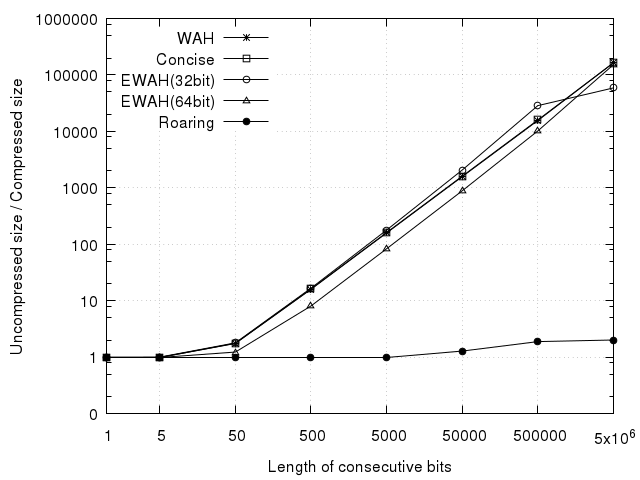
\includegraphics[width=\linewidth]{ratio.png}
\caption{Compression ratio}
\label{img:ratio}
\end{center}
\end{figure}

In the second part, we measured the performance of the compressed bitmaps working with the LTL formula. The first formula in the last experiment was chosen in this experiment: 

\begin{small}
$\mathop{G}((s_2 \mathrel{\rightarrow} \mathop{F}(\mathop{\neg}(s_1 \mathrel{U} s_2) \mathrel{W} (s_2 \mathrel{\vee} \mathop{G}s_1))) \mathrel{W} (\mathop{\neg}\mathop{F}(s_0 \mathrel{R} \mathop{X}s_2) \mathrel{W} ((s_0 \mathrel{\wedge} s_2 \mathrel{\wedge} \mathop{F}s_2) \mathrel{U} s_0)))$
\end{small}

It contains all 3 groups of operators and has 6 propositional logic operators, 6 temporal logic unary operators and 6 temporal logic binary operators. We also did a 10-cycles benchmark. In each cycle, the formula was executed with one group of input bitmaps from the last step and we recorded the time cost of each bitmap algorithm and each length of consecutive bits.

\begin{figure}[h]
\begin{center}
\centering
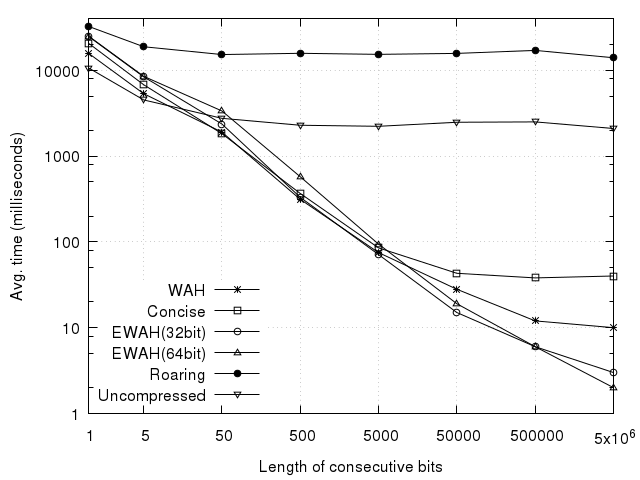
\includegraphics[width=\linewidth]{time.png}
\caption{Average time spent on the LTL formula}
\label{img:time}
\end{center}
\end{figure}

According to Figure \ref{img:time}, the performance of the RLE-model algorithms, WAH, EWAH and Concise is obviously relevant to $slen$, and EWAH is faster than the others when $slen > 5000$. Roaring bitmap and uncompressed bitmap demonstrate their $O(n)$ time complexities and the former is slower than the other.

%% }}} --- Subsection

%% }}} --- Section

\section{Conclusion and future work}\label{sec:conclusion} %% {{{

We proposed a solution of evaluating LTL formulas with bitmaps. The event states are mapped into bits of bitmaps which then are manipulated to implement the LTL operators. The performance benchmark of the fundamental operators and the complicated LTL formulas proved its feasibility.

To further exploit the potential of bitmap, we introduced bitmap compression algorithms in our solution and integrated them with our algorithms. In the experiments, as we expected, the compressed bitmap demonstrated its ability of compressing the sparse bitmaps and accelerating the LTL operations when there were certain amount of consecutive sequences.

This solution is designed only for the offline evaluation, and if we want to apply it on the online analysis there is still much work to do. And it is also very interesting to have the algorithms parallelized to treat huge amount of data.

%% }}} --- Section
